%%% MCCA stands for "Master-class of the Computer Archaeology"
\documentclass[t,aspectratio=169]{beamer}
\usetheme{CambridgeUS}
\usepackage[utf8]{inputenc}
\usepackage[english,russian]{babel}
\usepackage{amsmath,amsfonts, amsthm,amssymb}
\usepackage{dsfont}
%\usepackage{enumitem}

\usepackage{bbm}
\usefonttheme[onlymath]{serif}
\usepackage{graphicx}
\graphicspath{{./images}}
\usepackage{xlop}
\usepackage[absolute,overlay]{textpos}
\textblockorigin{10mm}{10mm} % start everything near the top-left corner
\usepackage{soul}
\newcounter{binst}
\makeatletter
\newcommand{\FormatBinary}[1]{\begingroup%
\setcounter{binst}{0}
\def\SOUL@soeverytoken{%
\stepcounter{binst}%
\ifnum\value{binst}=5\relax%
\setcounter{binst}{1}\,%
\fi%
\the\SOUL@token}%
\so{#1}\endgroup} 
\makeatother
\usepackage{booktabs}

\ExplSyntaxOn

\NewDocumentCommand{\binaryaddition}{mm}
 {
  \kartashuvit_binadd:nn { #1 } { #2 }
 }

\tl_new:N \l__kartashuvit_binadd_a_tl
\tl_new:N \l__kartashuvit_binadd_b_tl
\tl_new:N \l__kartashuvit_binadd_c_tl

\cs_new_protected:Nn \kartashuvit_binadd:nn
 {
  \tl_set:Nx \l__kartashuvit_binadd_c_tl
   {
    \int_to_bin:n { \int_from_bin:n { #1 } + \int_from_bin:n { #2 } }
   }
  % pad the summands with \scan_stop:
  \tl_set:Nx \l__kartashuvit_binadd_a_tl
   {
    \prg_replicate:nn
     { \tl_count:N \l__kartashuvit_binadd_c_tl - \tl_count:n { #1 } }
     { \scan_stop: }
    #1
   }
  \tl_set:Nx \l__kartashuvit_binadd_b_tl
   {
    \prg_replicate:nn
     { \tl_count:N \l__kartashuvit_binadd_c_tl - \tl_count:n { #2 } }
     { \scan_stop: }
    #2
   }
  \group_begin:
  \setlength{\tabcolsep}{3pt}
  \begin{tabular}{@{} c *{ \tl_count:N \l__kartashuvit_binadd_c_tl } { c } }
  \tl_map_function:NN \l__kartashuvit_binadd_a_tl \__kartashuvit_binadd_tab:n \\
  +
  \tl_map_function:NN \l__kartashuvit_binadd_b_tl \__kartashuvit_binadd_tab:n \\
  \midrule
  \tl_map_function:NN \l__kartashuvit_binadd_c_tl \__kartashuvit_binadd_tab:n \\
  \end{tabular}
  \group_end:
 }

\cs_new:Nn \__kartashuvit_binadd_tab:n { & #1 }

\ExplSyntaxOff

% I follow the circuitikz manual
% https://ctan.mirror.norbert-ruehl.de/graphics/pgf/contrib/circuitikz/doc/circuitikzmanual.pdf

\usepackage{circuitikz}
\usetikzlibrary{positioning}
\ctikzset{
    logic ports=ieee,
    logic ports/scale=0.7,
}
\tikzset{sr-ff/.style={flipflop, flipflop def={
    t1=S, t2=CP, t3=R, t4={\ctikztextnot{Q}},
    t6=Q, nd=1}},
}
\usepackage{tikz}
\usetikzlibrary{trees}
\usepackage{amsmath}

\usepackage{verbatim}
\usepackage{listings}

%\addtobeamertemplate{navigation symbols}{}{%
%    \usebeamerfont{footline}%
%    \usebeamercolor[fg]{footline}%
%    \hspace{1em}%
%    \insertframenumber/\inserttotalframenumber
%}

\newcommand{\backupbegin}{
   \newcounter{finalframe}
   \setcounter{finalframe}{\value{framenumber}}
}
\newcommand{\backupend}{
   \setcounter{framenumber}{\value{finalframe}}
}
\usepackage{url}

\author{Андрей Рабусов}
\date{28 марта 2023}
\title[Программирование]{Основы вычислительной техники\\
Друзи, JunOst}

\begin{document}
\begin{frame}
    \maketitle
\end{frame}

\begin{frame}
    \frametitle{Содержание}
    \tableofcontents[sectionstyle=show,subsectionstyle=show]
\end{frame}

\section*{Введение}
\begin{frame}
    \frametitle{Компьютеры сейчас и тогда}
    \begin{figure}
        \begin{centering}
            \only<1>{
                
\includegraphics[height=0.7\textheight]{iphone}
                % Credit: https://upload.wikimedia.org/wikipedia/commons/a/ad/IPhone_1st_Gen.svg
                \caption{iPhone, 1st gen.}
            }
            \only<2>{
                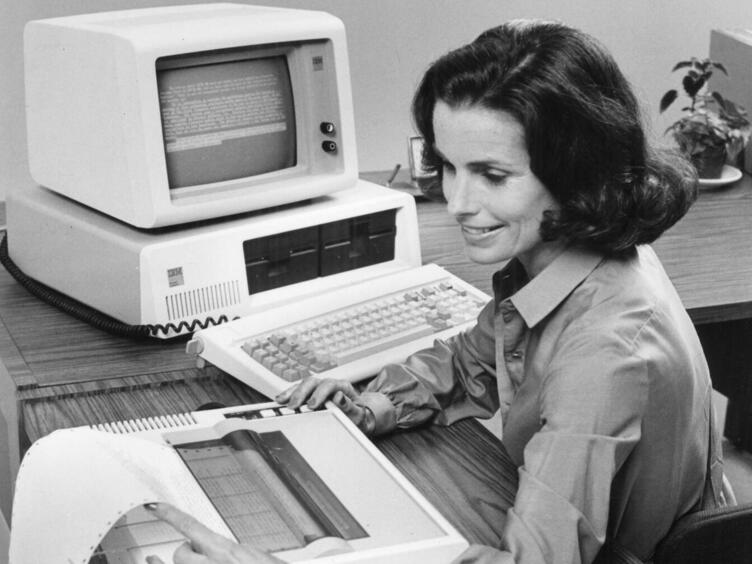
\includegraphics[height=0.7\textheight]{ibm-pc}
                % Credit: https://www.rheinpfalz.de/wirtschaft_artikel,-ein-pc-f%C3%BCr-18-000-dollar-_arid,5239259.html
                \caption{IBM PC}
            }
            \only<3>{
                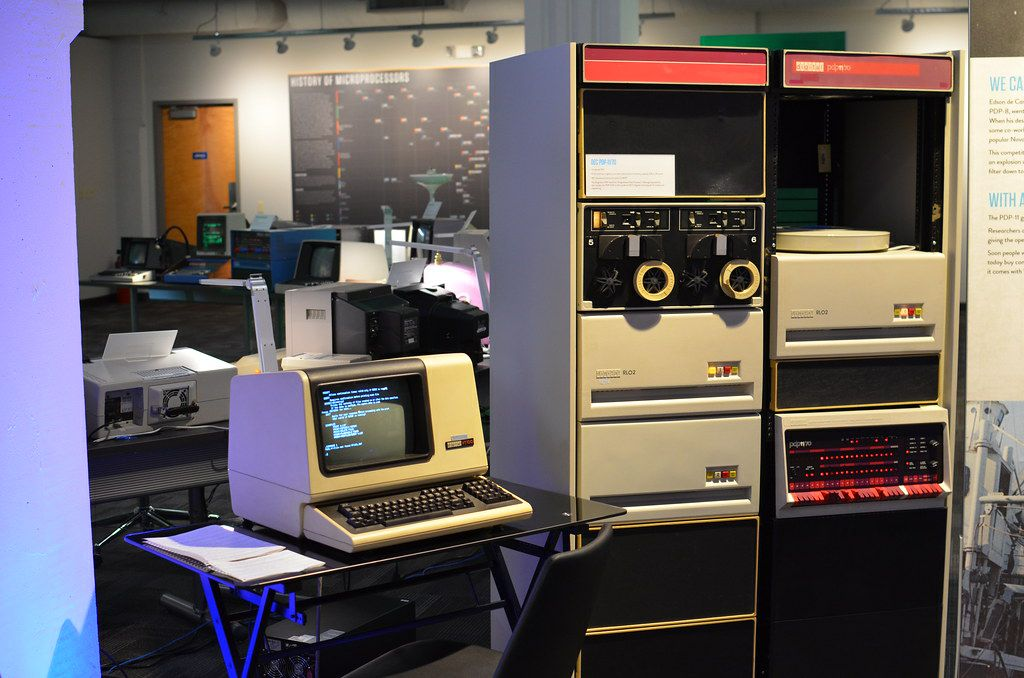
\includegraphics[height=0.7\textheight]{cm-pdp11}
                \caption{PDP-11/70}
            }
            \only<4>{
                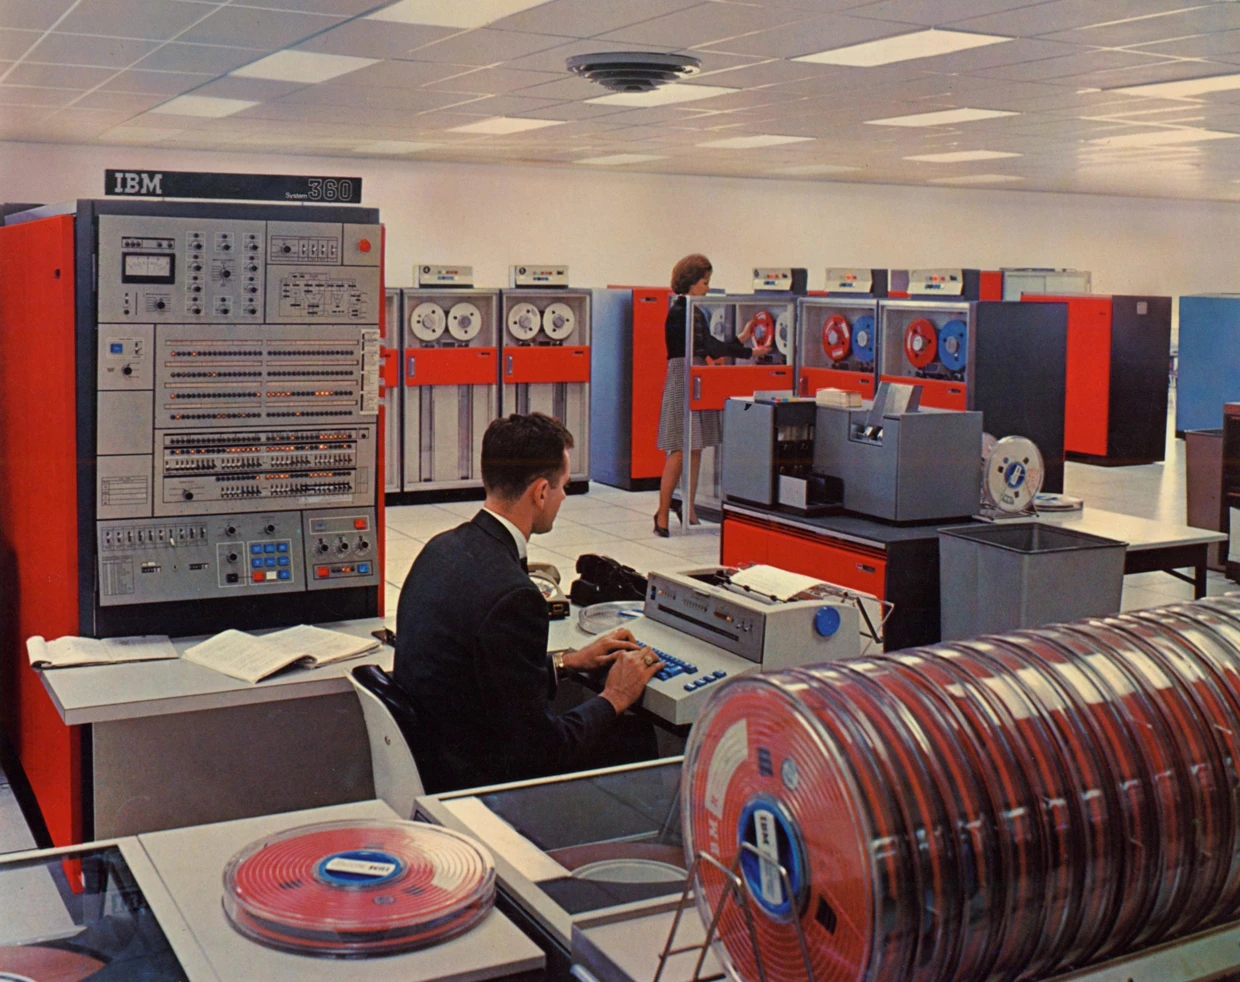
\includegraphics[height=0.7\textheight]{ibm-360}
                % Credit: https://media-cldnry.s-nbcnews.com/image/upload/t_fit-1240w,f_auto,q_auto:best/newscms/2014_19/432091/140509-ibm-360-mn-1120.jpg
                \caption{IBM 360}
            }
            \only<5>{
                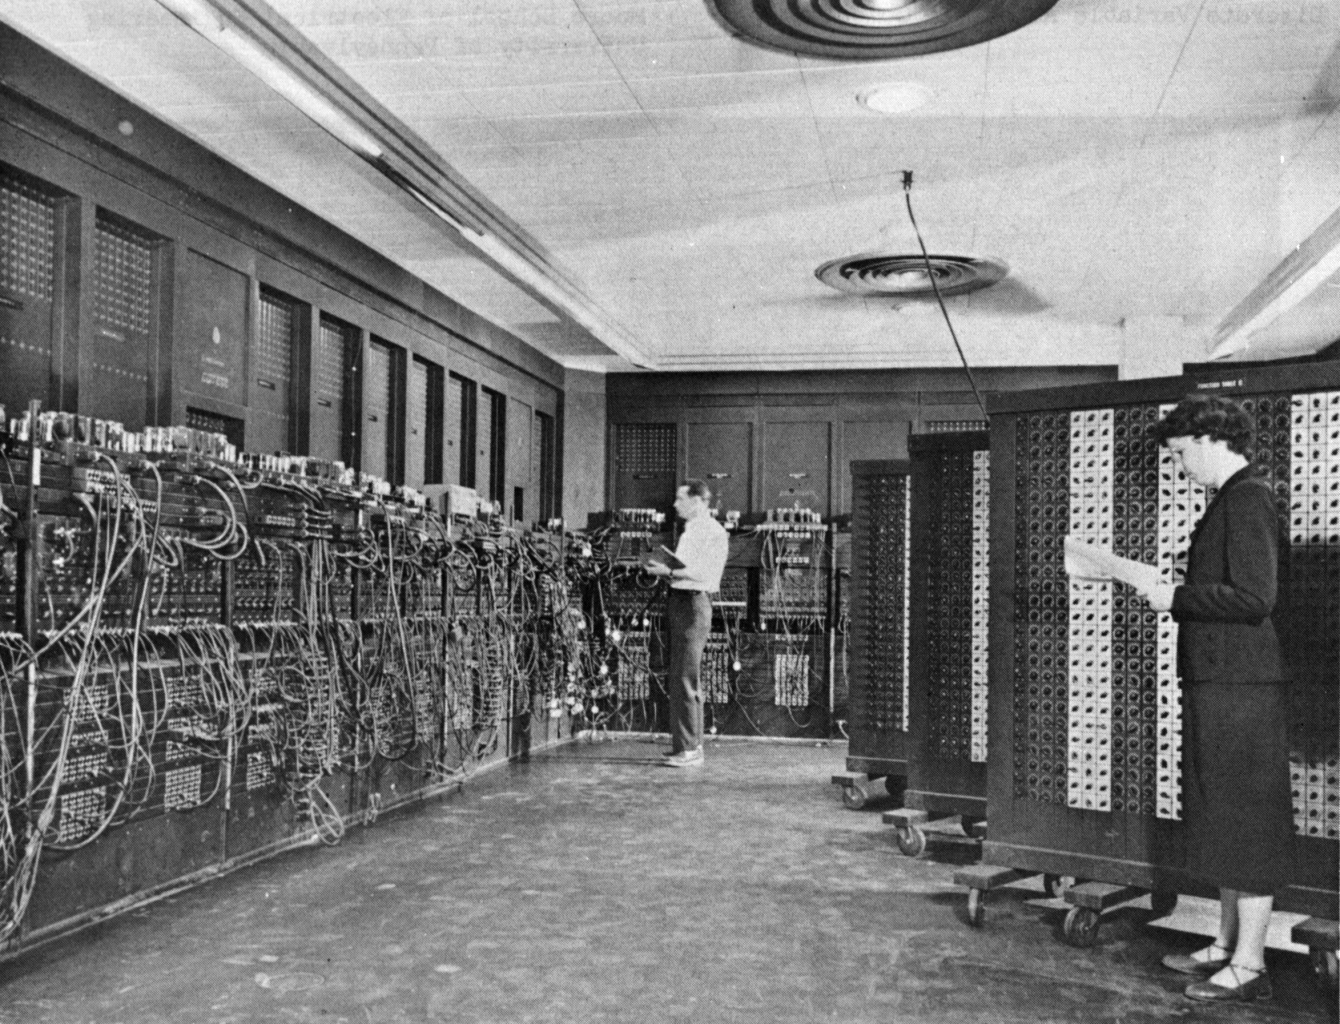
\includegraphics[height=0.7\textheight]{Eniac}
                % Credit: https://upload.wikimedia.org/wikipedia/commons/4/4e/Eniac.jpg
                \caption{Eniac}
            }
        \end{centering}
    \end{figure}

\end{frame}

\section{<<Железо>>}
\begin{frame}
    \frametitle{Двоичные числа}
    \only<1->{
    \begin{equation*}
        \FormatBinary{10110101}_2 =
        1\cdot 2^0 +
        0 \cdot 2^1 +
        1 \cdot 2^2 +
        0 \cdot 2^3 + 
        1 \cdot 2^4 + 
        0 \cdot 2^5 + 
        1 \cdot 2^6 + 
        1 \cdot 2^7 = 181
    \end{equation*}
    }\only<2->{
    \par\vspace{0.25cm}
    \begin{minipage}{0.75\textwidth}
        Сложение чисел в обычной (десятеричной) системе:
    \end{minipage}
    \begin{minipage}{0.24\textwidth}
        \opadd{384}{56}\qquad\par\vspace{0.5cm}
    \end{minipage}
    }\only<3->{
    \begin{minipage}{0.75\textwidth}
        Сложение чисел в двоичной системе:
    \end{minipage}
    \begin{minipage}{0.24\textwidth}
        \binaryaddition{1010}{1001}\qquad\par
    \end{minipage}
    }
\end{frame}

\begin{frame}
    \frametitle{Логические операции}
    \begin{columns}
        \begin{column}{0.49\textwidth}
            \only<1->{
                \begin{minipage}{0.69\textwidth}
                    \begin{equation*}
                        \begin{array}{c|c}
                            \toprule
                            x & \mathrm{not}\;x\\
                            \hline
                            0 & 1 \\
                            1 & 0 \\
                            \bottomrule
                        \end{array}
                    \end{equation*}
                \end{minipage}
            }\only<2->{
                \begin{minipage}{0.19\textwidth}
                    \begin{tikzpicture}[scale=0.1]
                        \node[ieeestd not port] (not1) at (0,0) {not};
                    \end{tikzpicture}
                \end{minipage}
            }\only<3->{
                \par\vspace{1.0cm}
                \begin{minipage}{0.69\textwidth}
                    \begin{equation*}
                        \begin{array}{c|c|c}
                            \toprule
                            x & y & x\;\mathrm{and}\;y \\
                            \hline
                            0 & 0 & 0 \\
                            1 & 0 & 0 \\
                            0 & 1 & 0 \\
                            1 & 1 & 1 \\
                            \bottomrule
                        \end{array}
                    \end{equation*}
                \end{minipage}
            }\only<4->{
                \begin{minipage}{0.19\textwidth}
                    \begin{tikzpicture}[scale=0.1]
                        \node[ieeestd and port] (and1) at (0,0) {and};
                    \end{tikzpicture}
                \end{minipage}
            }
        \end{column}

        \begin{column}{0.49\textwidth}
            \only<5->{
                \begin{minipage}{0.69\textwidth}
                    \begin{equation*}
                        \begin{array}{c|c|c}
                            \toprule
                            x & y & x\;\mathrm{or}\;y \\
                        \hline
                        0 & 0 & 0 \\
                        1 & 0 & 1 \\
                        0 & 1 & 1 \\
                        1 & 1 & 1 \\
                        \bottomrule
                    \end{array}
                \end{equation*}
            \end{minipage}
        }\only<6->{
            \begin{minipage}{0.19\textwidth}
                \begin{tikzpicture}[scale=0.1]
                    \node[ieeestd or port] (or1) at (0,0) {or};
                \end{tikzpicture}
            \end{minipage}
        }\only<7->{
            \par\vspace{1.0cm}
            \begin{minipage}{0.69\textwidth}
                \begin{equation*}
                    \begin{array}{c|c|c}
                        \toprule
                        x & y & x\;\mathrm{xor}\;y \\
                        \hline
                        0 & 0 & 0 \\
                        1 & 0 & 1 \\
                        0 & 1 & 1 \\
                        1 & 1 & 0 \\
                        \bottomrule
                    \end{array}
                \end{equation*}
            \end{minipage}
        }\only<8->{
            \begin{minipage}{0.19\textwidth}
                \begin{tikzpicture}[scale=0.1]
                    \node[ieeestd xor port] (xor1) at (0,0) {xor};
                \end{tikzpicture}
            \end{minipage}
        }
        \end{column}
    \end{columns}
\end{frame}

\begin{frame}
    \frametitle{Арифметические операции: half-adder}
    Сумма двух битов: $\overline{CS} = s = x + y$\par
    \begin{minipage}{0.69\textwidth}
        \begin{equation*}
            \begin{array}{c|c|c|c}
                \toprule
                x & y & S & C \\
                \hline
                0 & 0 & 0 & 0 \\
                1 & 0 & 1 & 0 \\
                0 & 1 & 1 & 0 \\
                1 & 1 & 0 & 1 \\
                \bottomrule
            \end{array}
        \end{equation*}
    \end{minipage}
    \only<2>{
        \begin{minipage}{0.19\textwidth}
            %https://tex.stackexchange.com/questions/301295/circuitikz-parallel-logic-gate-wiring
            \begin{circuitikz}[scale=0.9]
                \draw (0, 4)node[xor port] (xorone){xor}
                (0, 2)node[and port] (and){and}
                (xorone.in 1) node[left=0.5cm](a) {A}
                (xorone.in 2) node[left=0.5cm](b) {B}
                (xorone.out) node[right=0.1cm](s) {S}
                (and.out) node[right=0.1cm](c) {C}

                (a.east) to[short,-*] (xorone.in 1) |- (and.in 1)
                (b.east) to[short,-*] ($(b.east)!.5!(xorone.in 2)$) coordinate (branch)
                -- (xorone.in 2)
                (branch) |- (and.in 2);
            \end{circuitikz}
        \end{minipage}
        }
\end{frame}

\begin{frame}
    \frametitle{Full adder}
    \begin{circuitikz}[scale=0.9]
        \node[xor port] (xorone) {xor};
        \node[and port, below=of xorone] (andone) {and};
        \node[left=of xorone.in 1] (a) {A};
        \node[left=of xorone.in 2] (b) {B};

        \draw
        (a.east) to[short,-*] (xorone.in 1) |- (andone.in 1)
        (b.east) to[short,-*] ($(b.east)!.5!(xorone.in 2)$) coordinate (branch)
        -- (xorone.in 2)
        (branch) |- (andone.in 2);

        \node[xor port, right=of xorone, anchor=in 1] (xortwo){xor};
        \node[and port] (andtwo) at (xortwo |- andone.in 1) {and};
        \draw
        (xorone.out) to[short,-*] (xortwo.in 1) |- (andtwo.in 1);

        \node[or port, right=2cm of andtwo.in 2, anchor=in 1] (or) {or};
        \draw (andtwo.out) |- (or.in 1);

        \node[right=0.1cm of or.out] (C) {$\mathrm{C}_\mathrm{out}$};
        \node (S) at (C |- xortwo.out) {S};

        \node (mid1) at ($(xorone.in 2)!.5!(andone.in 1)$) {};
        \node[left=of mid1] (cin) {$\mathrm{C}_\mathrm{in}$};
        \node (mid2) at ($(xorone.out)!.5!(andone.out)$) {};
        \draw (cin) to[short,-*] (mid2) |- (xortwo.in 2);
        \draw (mid2) |- (andtwo.in 2);
        \draw (andone.out)|- (or.in 2);
        \draw (xortwo.out) -- (S);
    \end{circuitikz}
\end{frame}

\begin{frame}
    \frametitle{Логические вентили: кирпичи в компьютерах}
    \begin{minipage}{0.85\textwidth}
        \begin{figure}
            \begin{centering}
                %Credit: https://preview.redd.it/acnsw84ozyu61.png
                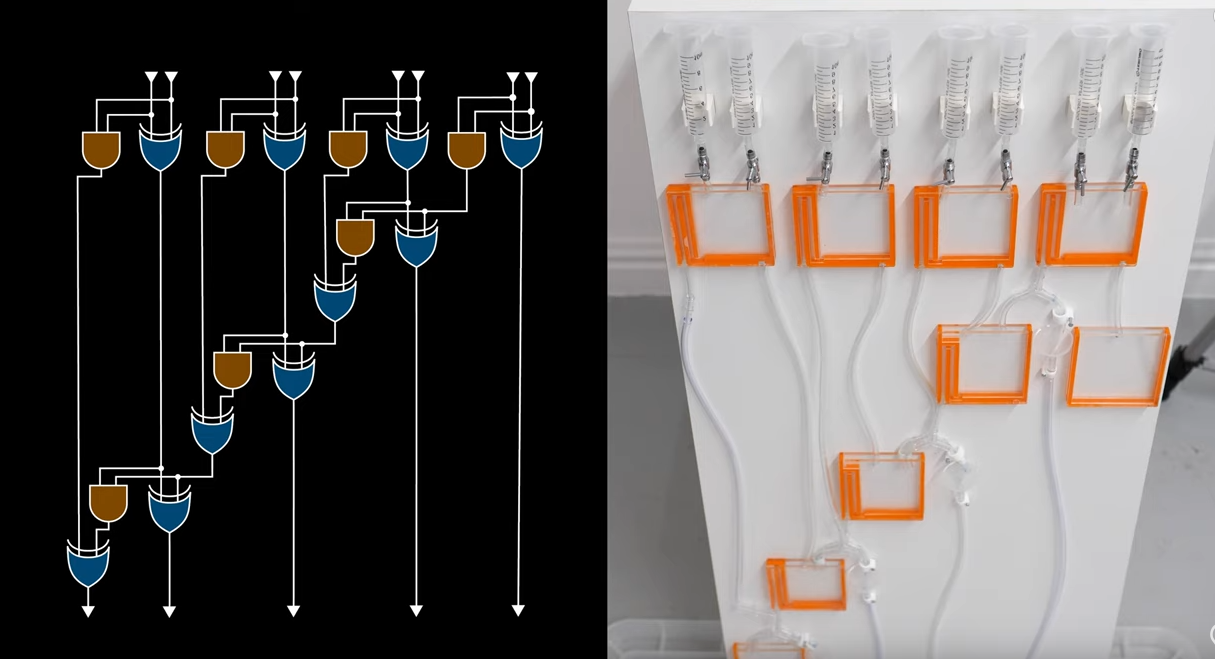
\includegraphics[height=0.7\textheight]{water-adder}
                \caption{Четырёхбитный сумматор}
            \end{centering}
        \end{figure}
    \end{minipage}
    \begin{minipage}{0.14\textwidth}
        Youtube:
        
\includegraphics[width=0.9\textwidth]{water-adder-qr}
    \end{minipage}
\end{frame}

\begin{frame}
    \frametitle{Делаем логические вентили из транзисторов}
    %Credit: https://gist.github.com/xarantolus/fa2bb75becf410fdc9929466ba8b5ed8
    \only<1>{
        \begin{figure}
            \begin{centering}
        \begin{circuitikz}[scale=0.9]
            \draw (3,3) node[npn](npn1) {} ;
            \draw (0,3) node[left=0.5cm] {$Q$};
            \draw (0,3) to[short, o-] (0.5, 3) to[R=$15K$] (npn1.base) node[anchor=east]{};
            \draw (3,6) to[short,o-,l_=$5V$] (3,5.5) to[R=$1K$] node[short](outConn) {} (npn1.collector) node[anchor=south] {};
            \draw (npn1.emitter) node[anchor=north] {} to[short] node[ground] {} (3,2);
            \draw (outConn) to[short, *-o] ++(2, 0)
            node[right=0.2cm]{$\overline{Q}$};
        \end{circuitikz}
                \caption{NOT gate}
            \end{centering}
        \end{figure}
    }\only<2>{
          % derived from this image: http://www.play-hookey.com/digital_electronics/images/rtl-nor4t.gif
   \begin{figure}[h!]
    \begin{center}
      \begin{circuitikz}
        \draw (0.5,3) node[npn](npn1) {};
        \draw (3,3) node[npn](npn2) {};

        \draw (npn1.collector) to[short, -*] (npn2.collector);

        \draw (3,6) to[short,o-,l_=$3.6V$] (3,5.5) to[R=$640$] node[short](outConn) {} (npn2.collector) node[anchor=south] {};

        \draw (npn1.base) to[R, n=r1] ++(0, -1.5) to[short, -o] node[below]{$IN_1$} ++(0, -0.5);
        \draw (npn2.base) to[R, n=r2] ++(0, -1.5) to[short, -o] node[below]{$IN_2$} ++(0, -0.5);

        \draw (r1.s) node[left]{$470$};
        \draw (r2.s) node[left]{$470$};

        % Grounds
        \draw (npn1.emitter) node[anchor=north] {} to[short] node[ground] {} (0.5,2);
        \draw (npn2.emitter) node[anchor=north] {} to[short] node[ground] {} (3,2);

        \draw (outConn) to[short, *-o] node[right]{$OUT$} ++(2, 0);
      \end{circuitikz}
      \caption{RTL NOR}
    \end{center}
  \end{figure}
    }
\end{frame}

\begin{frame}
    \frametitle{Как запоминает компьютер? Статическая память}
    \begin{columns}
        \begin{column}{0.49\textwidth}
            %%% Taken from: https://latexdraw.com/draw-sr-flip-flop-with-circuitikz/
            \begin{tikzpicture}[scale=0.5]

                % AND logic gates
                \node[ieeestd and port] (and1) at (0,2) {AND};
                \node[ieeestd and port] (and2) at (0,-2) {AND};

                % NOR logic gates
                \draw (and1.out) -- ++(2.5,0) node[ieeestd nor port,
                anchor=in 1] (nor1) {NOR};
                \draw (and2.out) -- ++(2.5,0) node[ieeestd nor port,
                anchor=in 2] (nor2) {NOR};

                \draw (nor1.in 2) -| ++ (-0.2,-0.85) -- ++(3,-1.5) coordinate(a) |- (nor2.out);
                \draw (nor2.in 1) -| ++ (-0.2,0.85) -- ++(3,1.5) |- (nor1.out);

                % Labels
                \draw (and1.in 1) -- ++(-0.75,0) node[left]{R};
                \draw (and2.in 2) -- ++(-0.75,0) node[left]{S};
                \draw (and1.in 2) -- (and2.in 1)node[midway](clk){};
                \draw (clk.center) -- ++(-0.75,0) node[left]{Clk};

                \draw (nor1.out -| a) -- ++(0.75,0) node[right]{Q(t)};
                \draw (nor2.out -| a) -- ++(0.75,0) node[right]{Q(t)$^{'}$};

            \end{tikzpicture}
        \end{column}
        \begin{column}{0.49\textwidth}
            \only<2>{
            \begin{circuitikz}[]
                \draw (0,0) node[sr-ff](FF){} (FF.bup)
                node[above]{SR-FF};
                \draw (FF.pin 1) -- ++(-1,0) node[and port,
                anchor=out](AND1){}
                (FF.pin 3) -- ++(-1,0) node[and port,
                anchor=out](AND2){};
            \end{circuitikz}
        }
        \end{column}
    \end{columns}
\end{frame}

\begin{frame}
    \frametitle{Магнитные сердечники}
    % Credit: Wikipedia
    \begin{figure}
        \begin{centering}
    \only<1>{
        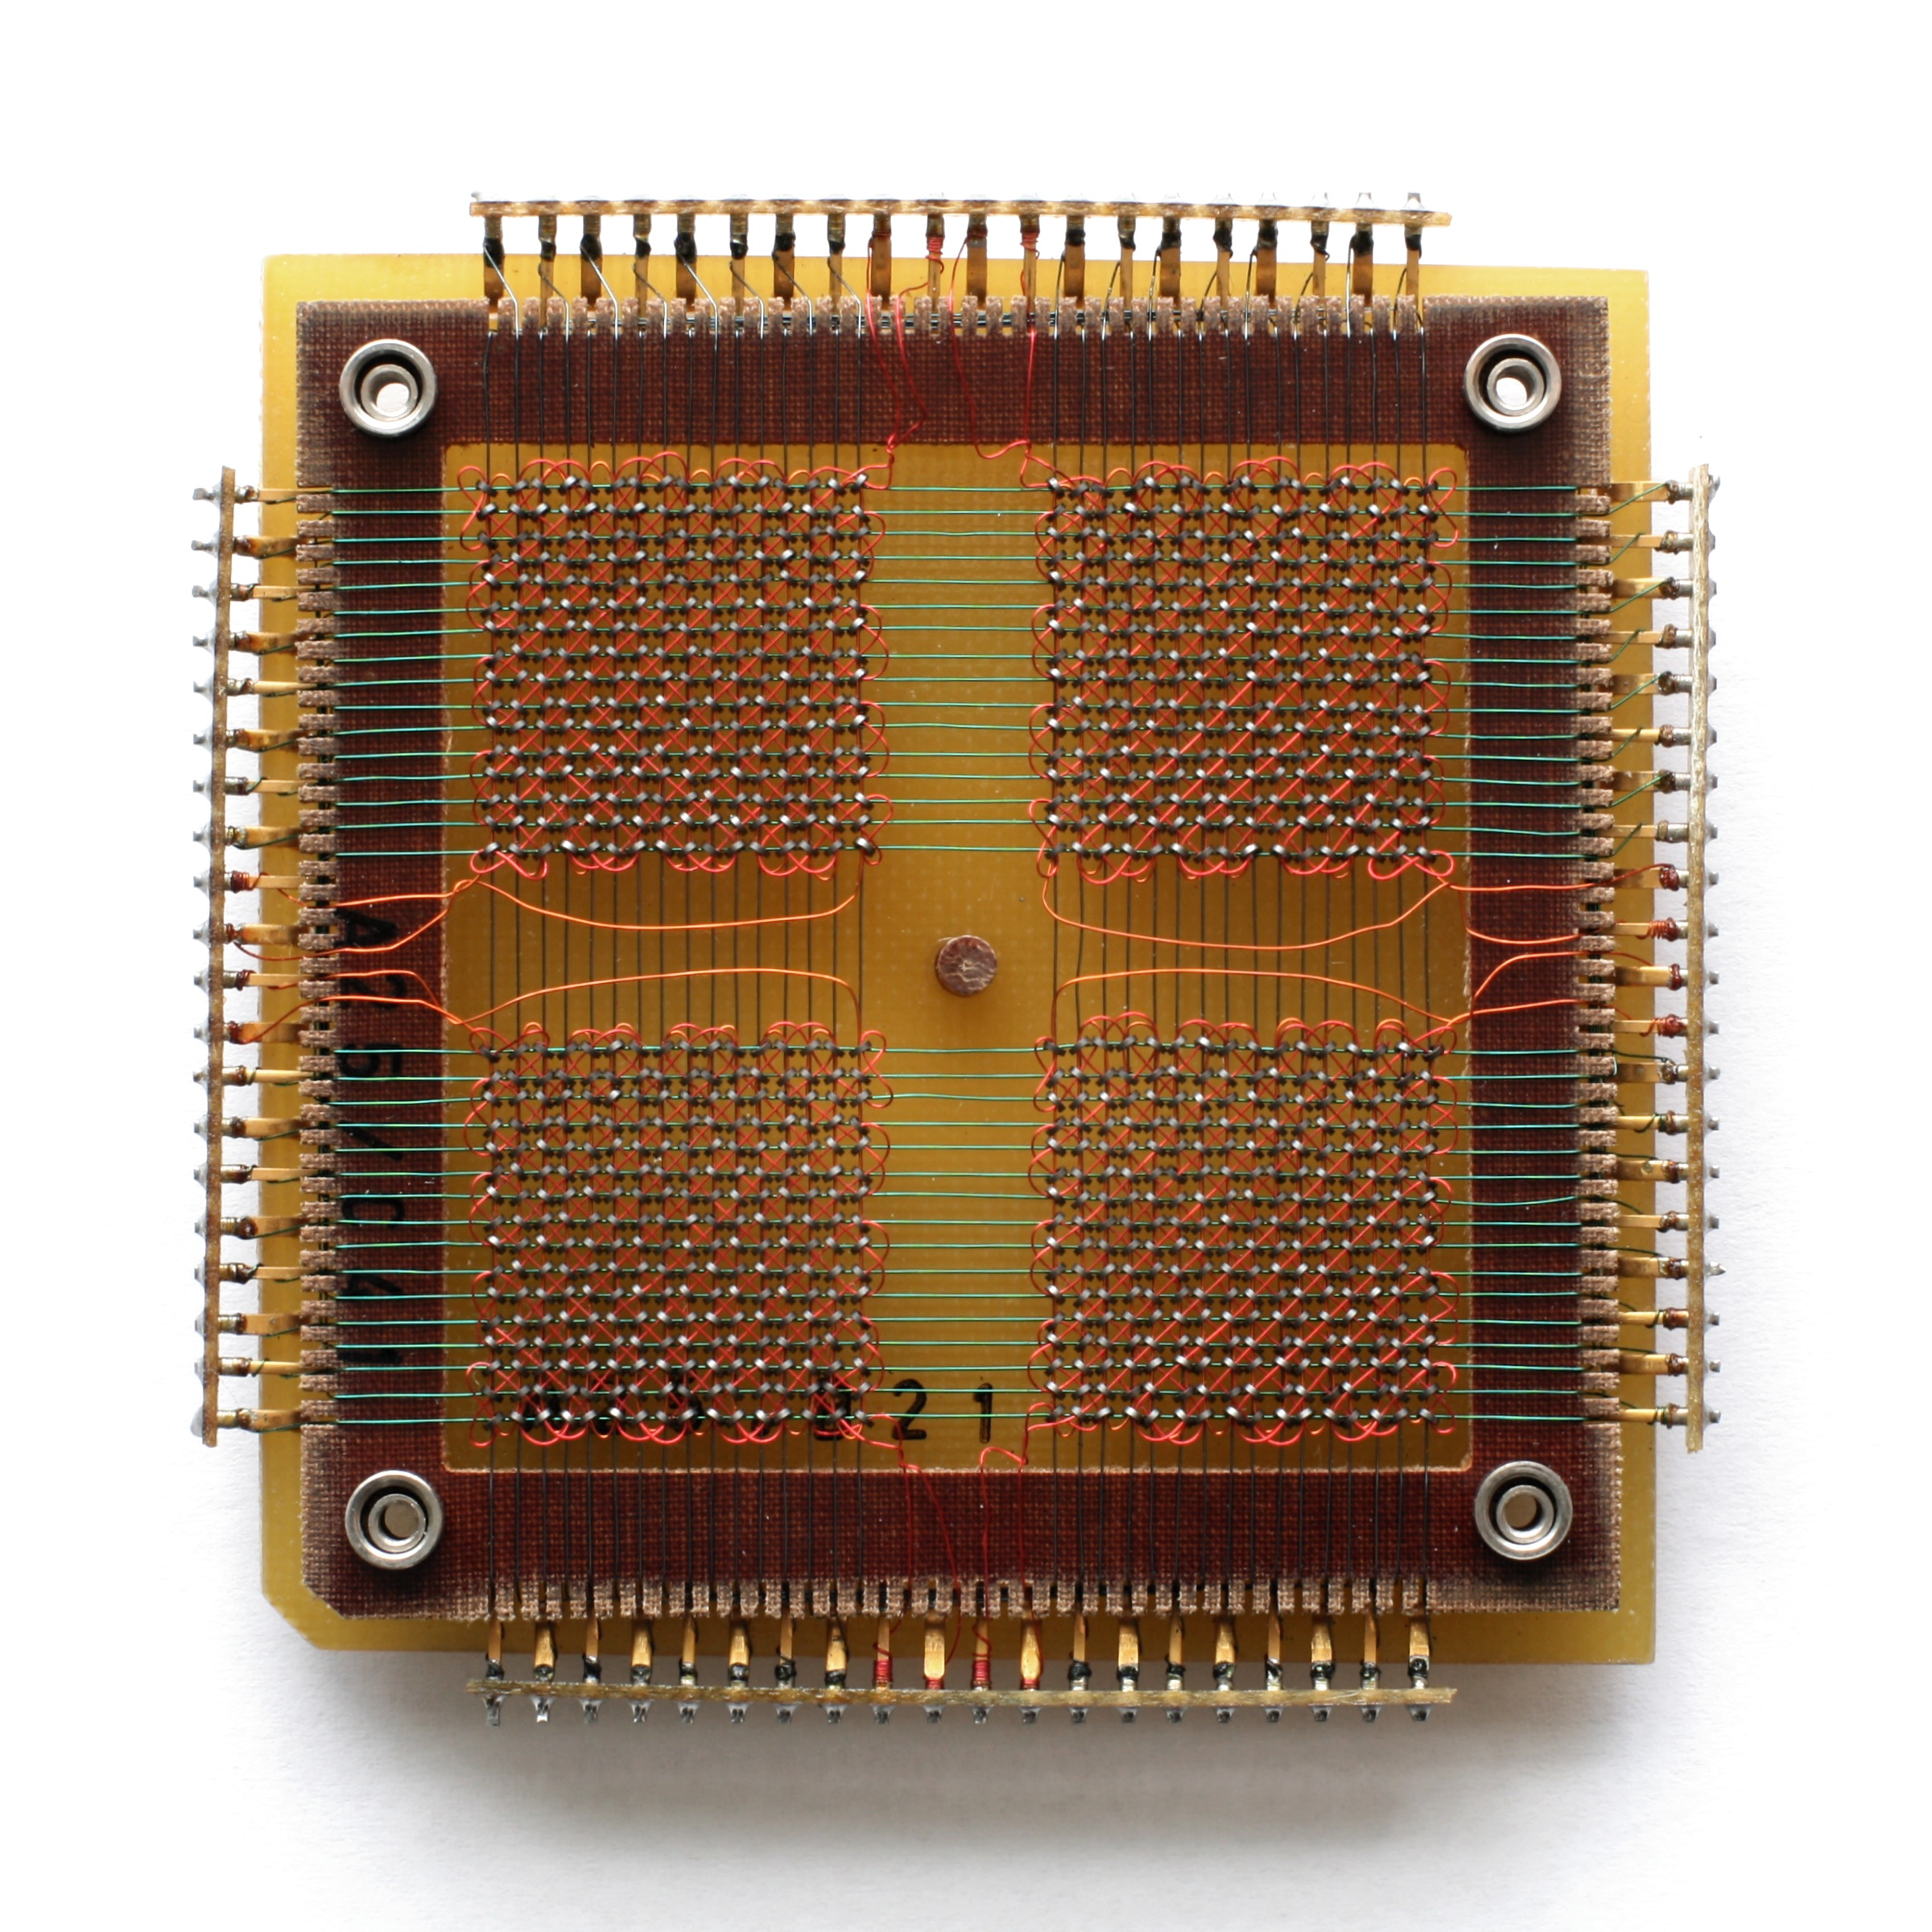
\includegraphics[height=0.8\textheight]{core-memory}
    }
    \only<2>{
        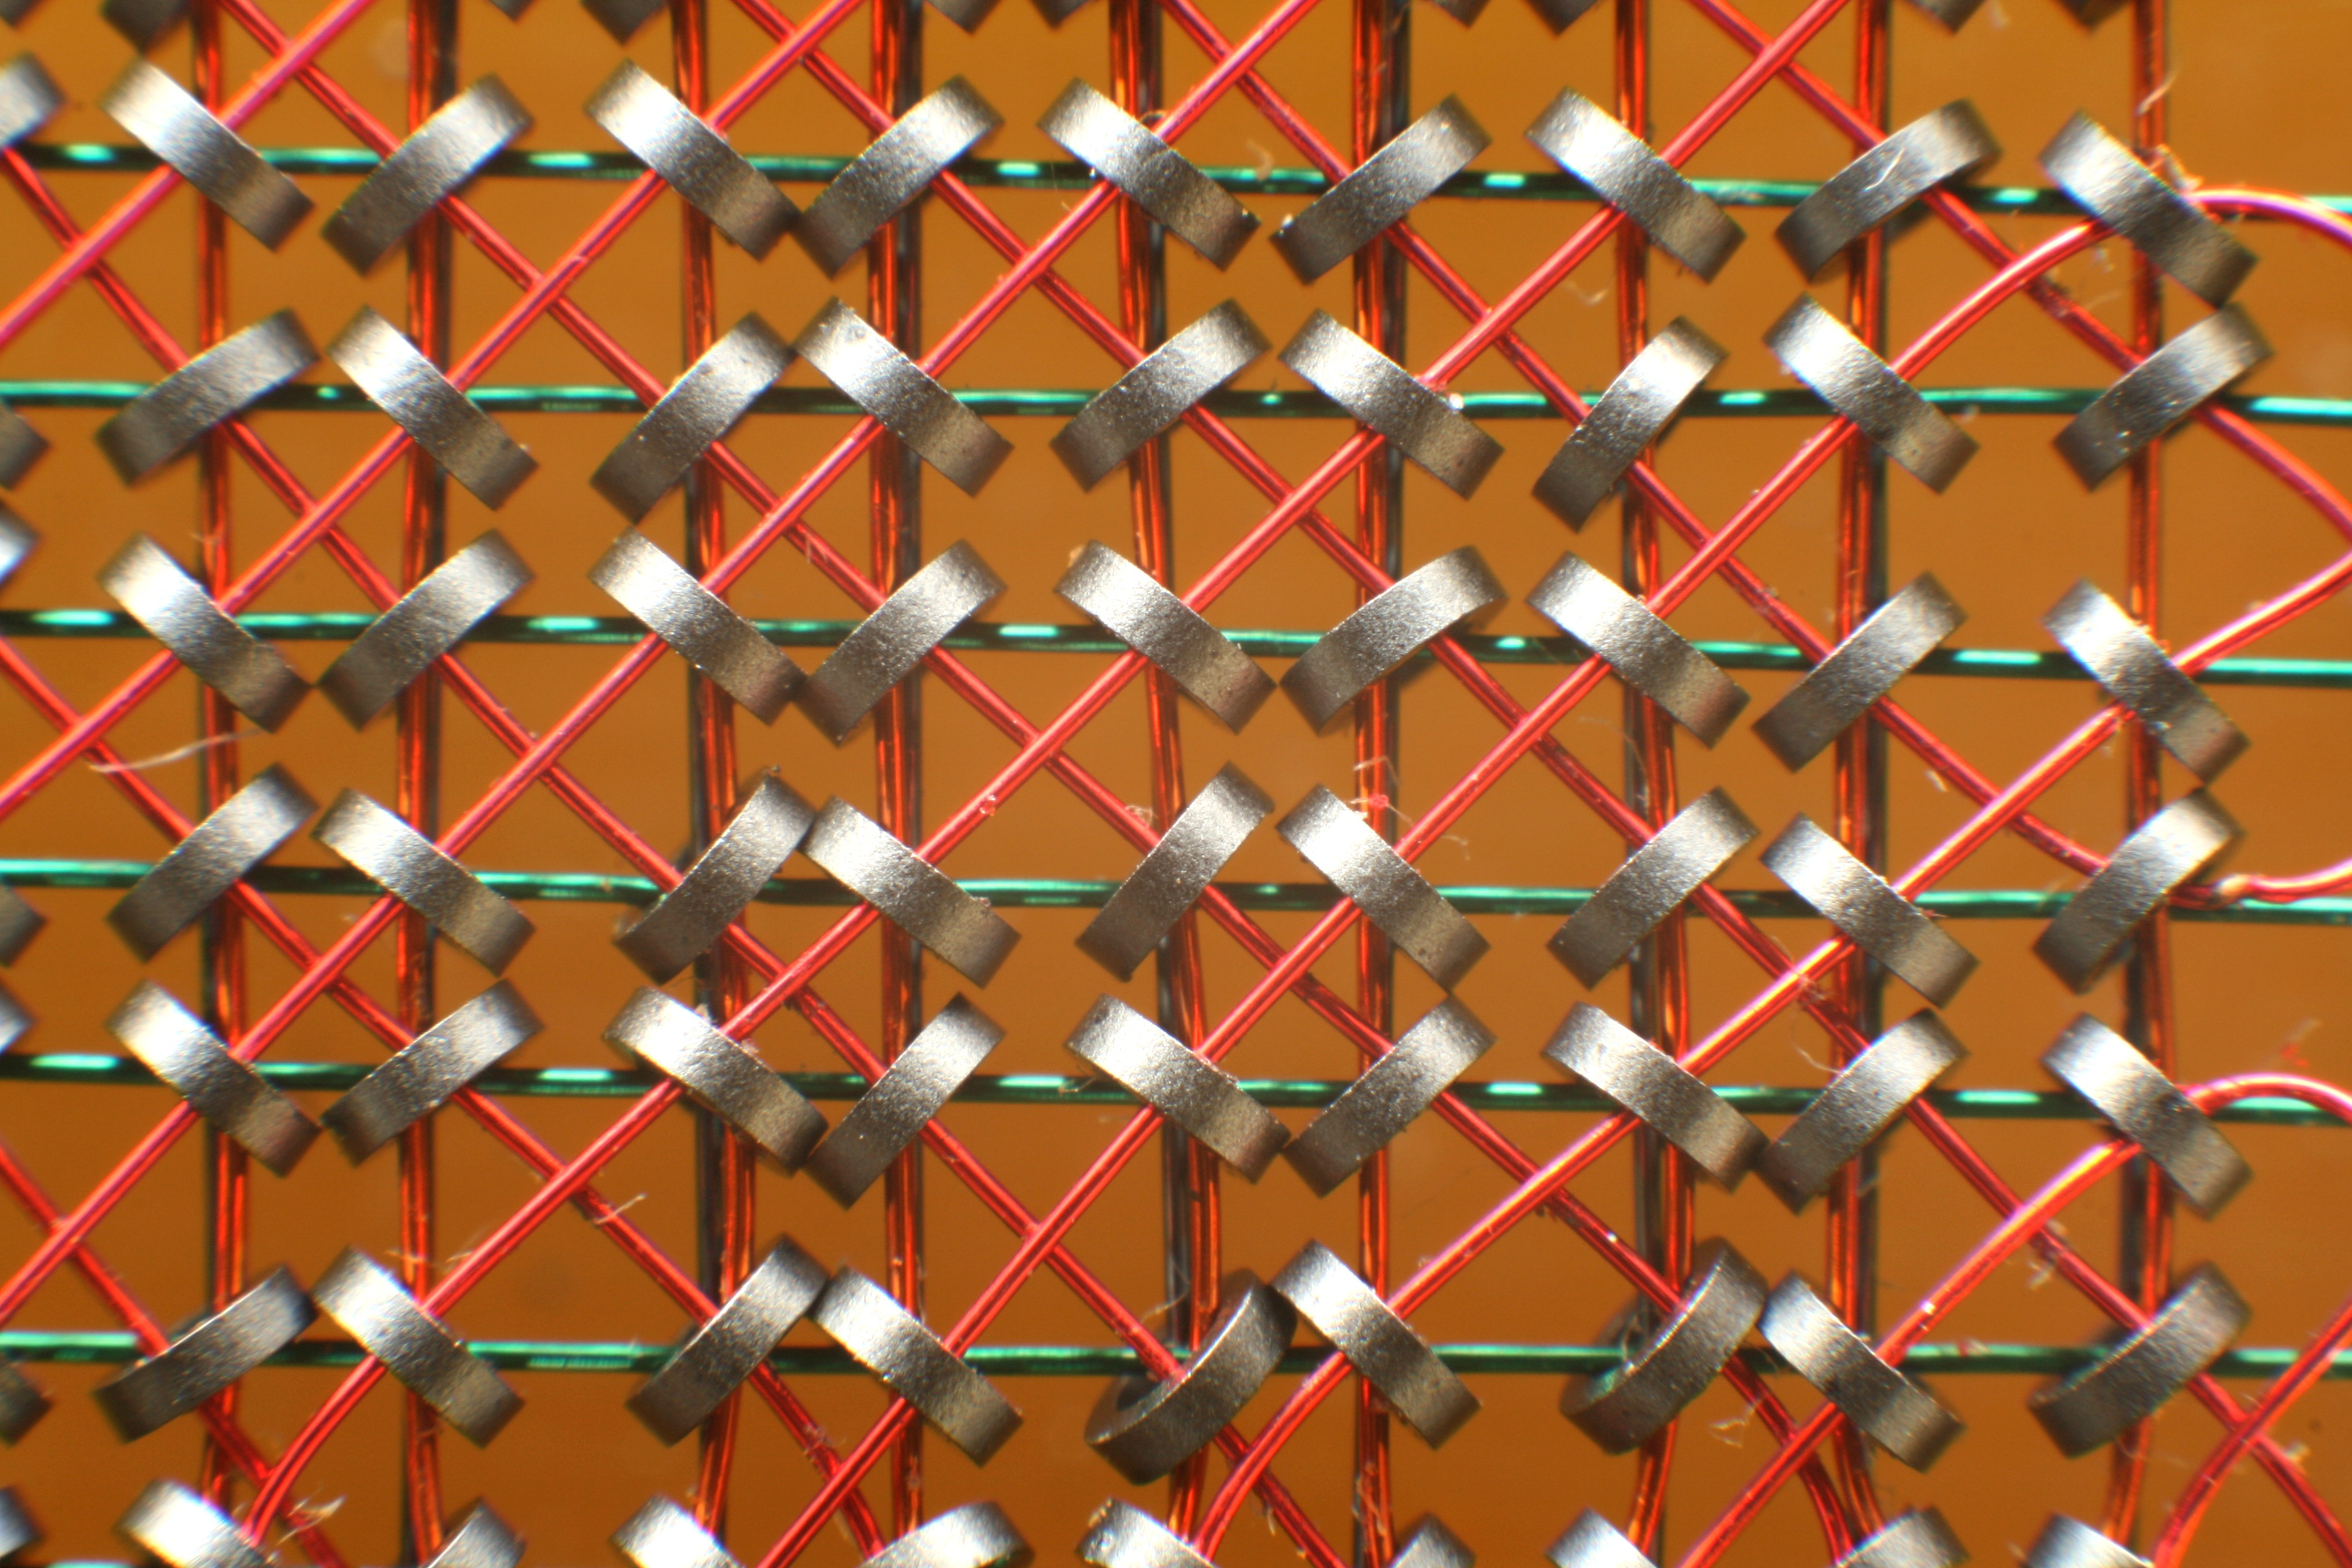
\includegraphics[height=0.8\textheight]{core-memory-zoomed-in}
    }
        \end{centering}
    \end{figure}
\end{frame}

\begin{frame}
    \frametitle{Динамическая память}
    % Credit: Wikipedia
    \begin{figure}
        \begin{centering}
            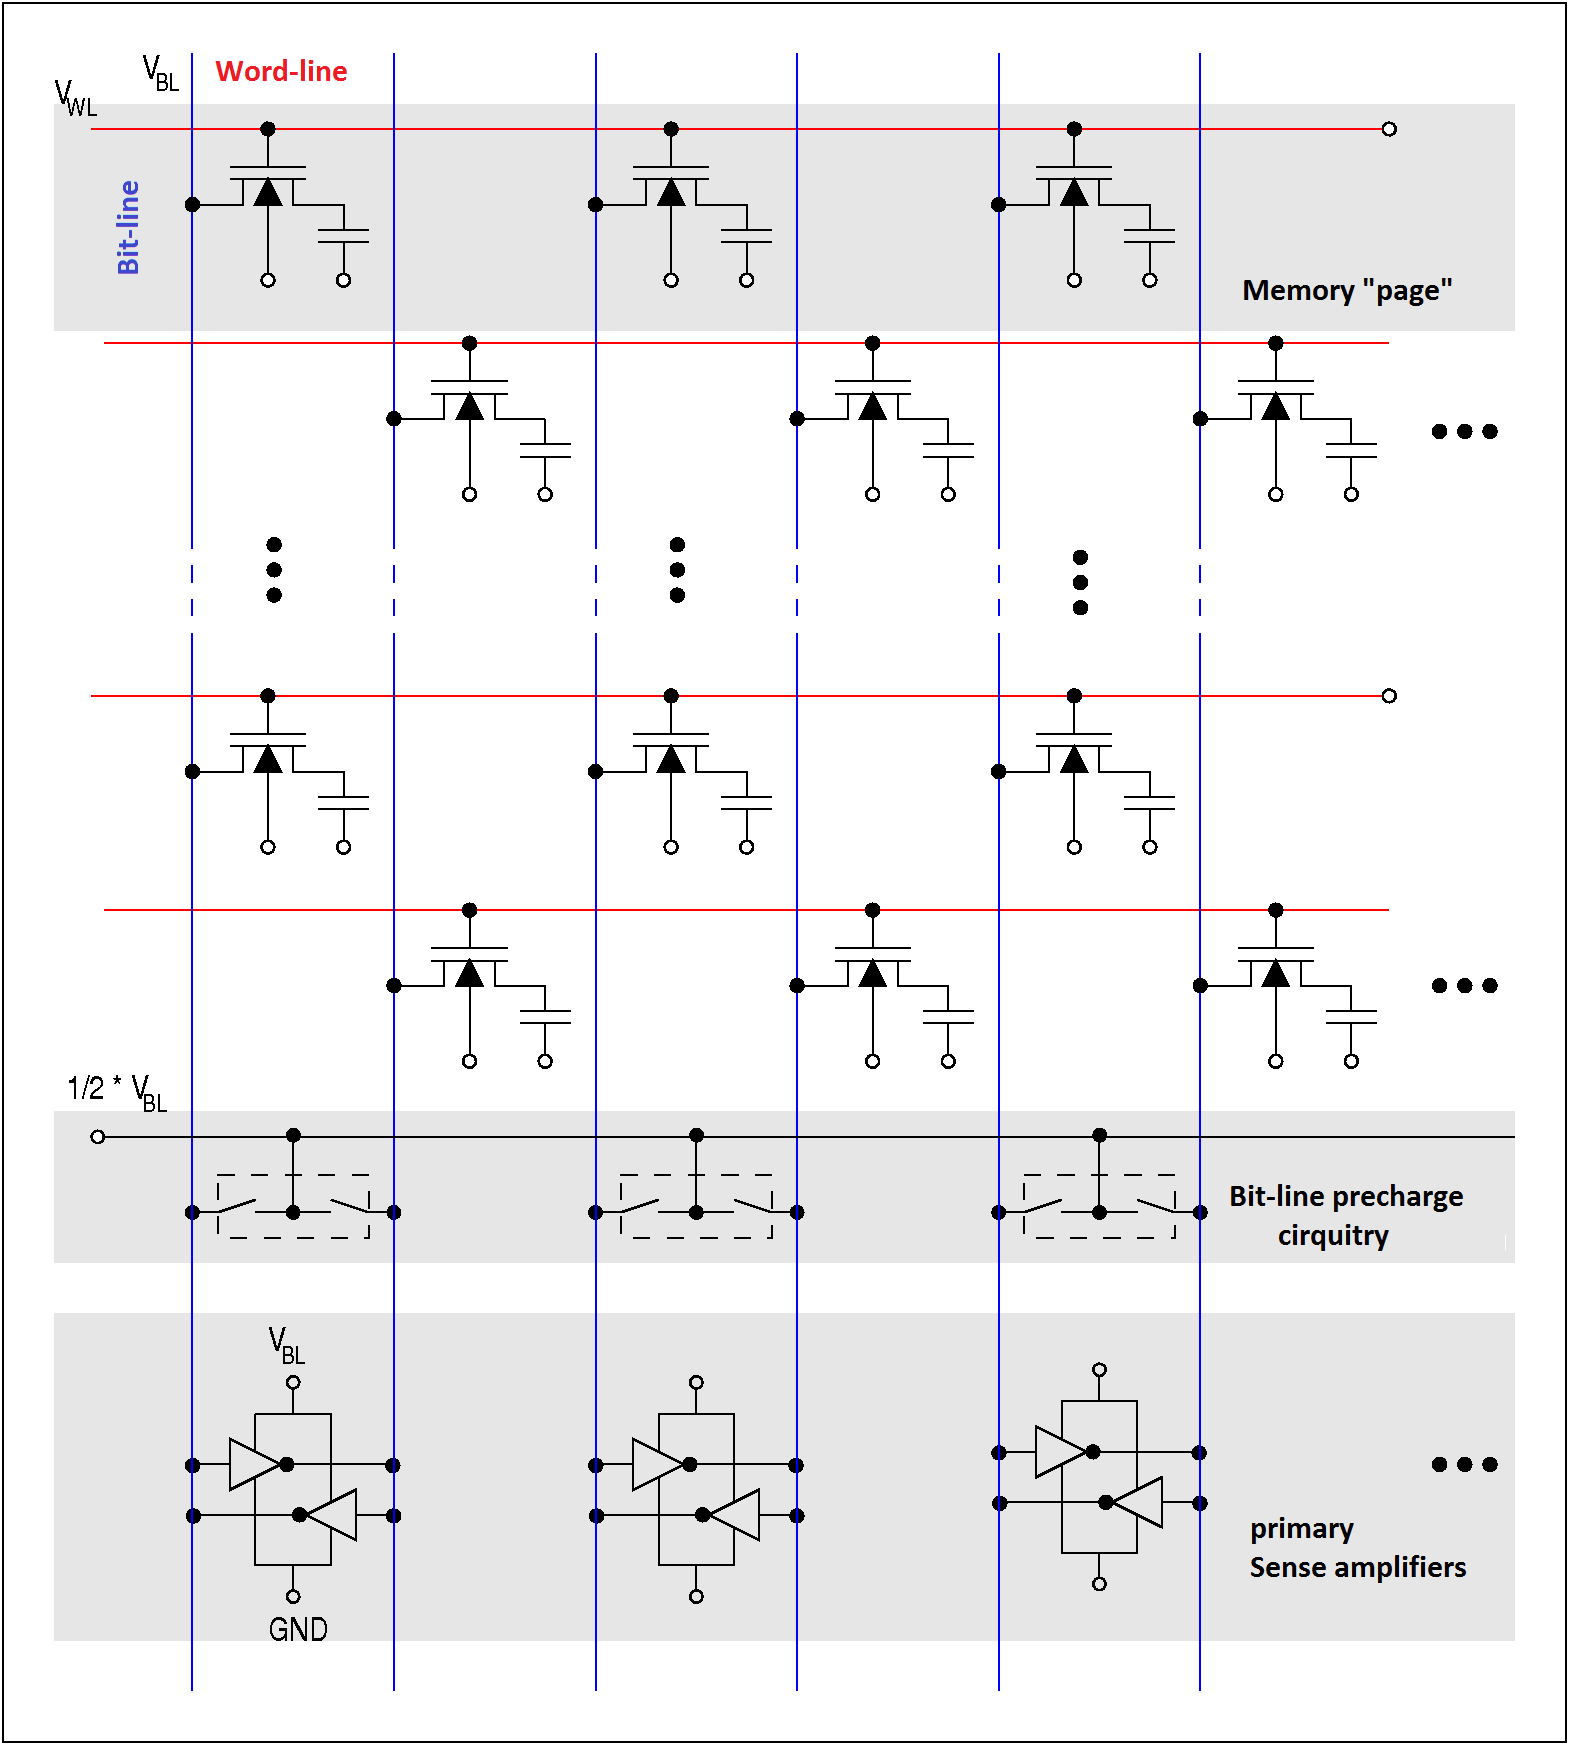
\includegraphics[height=0.8\textheight]{dram}
        \end{centering}
    \end{figure}
\end{frame}

\section{Взаимодействие человек--машина}
\begin{frame}
    \frametitle{Переключатели на передней панели}
    \begin{minipage}{0.8\textwidth}
        \begin{centering}
            %Credit: BlinkenBone
            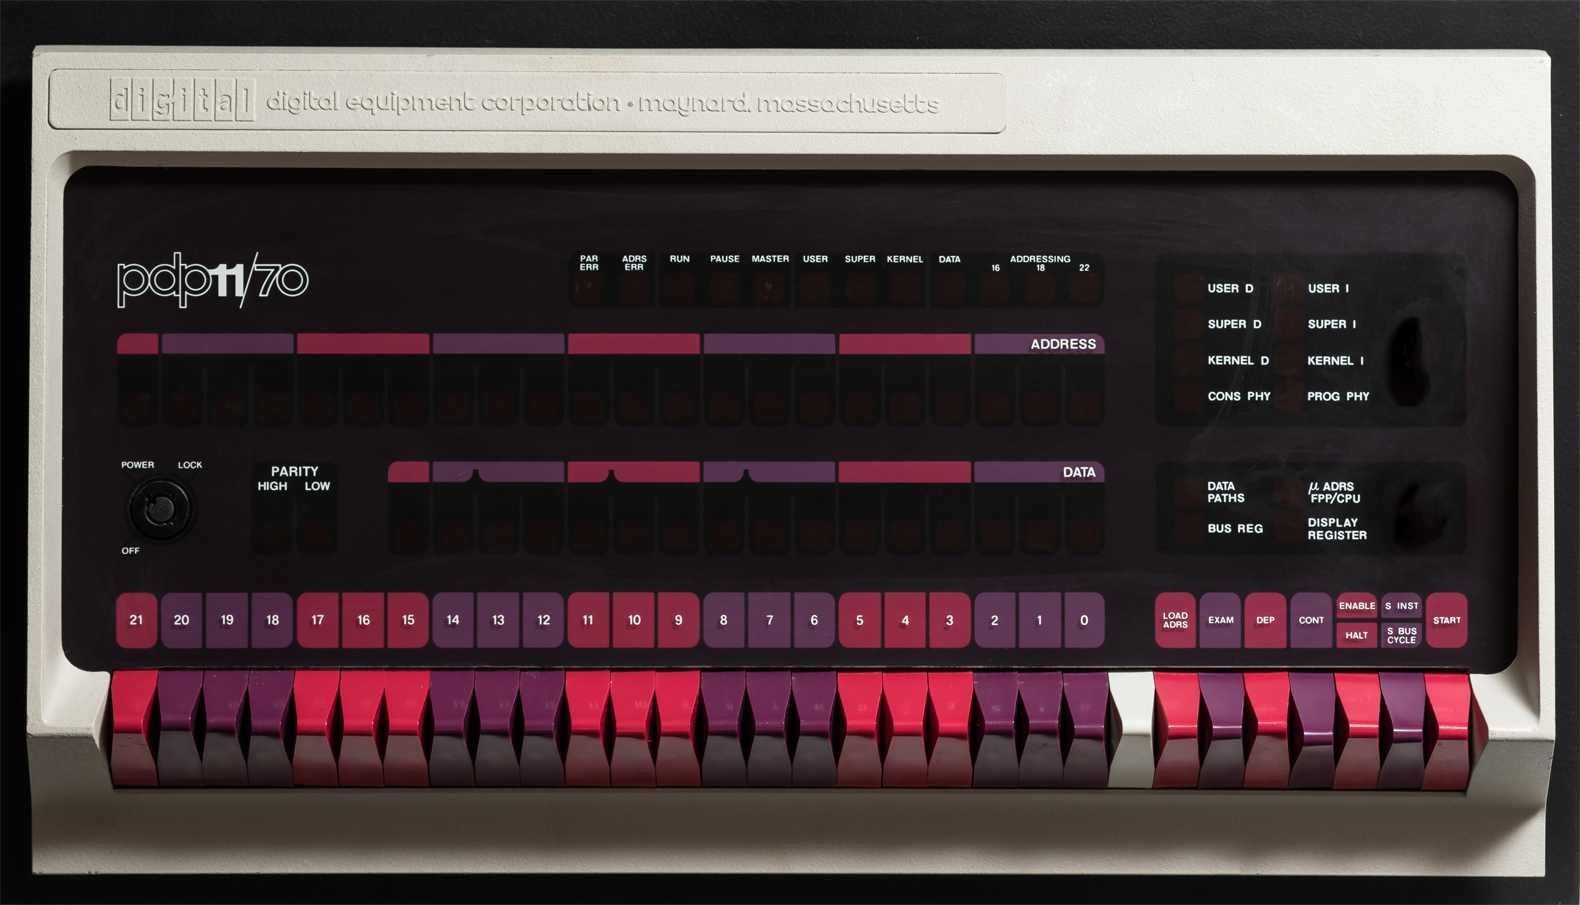
\includegraphics[width=0.97\textwidth]{pdp1170-fp}
        \end{centering}
    \end{minipage}
    \begin{minipage}{0.19\textwidth}
            
\includegraphics[width=0.97\textwidth]{js-pdp11}
    \end{minipage}
\end{frame}

\begin{frame}
    \frametitle{Перфокарты}
    \begin{figure}
        \begin{centering}
            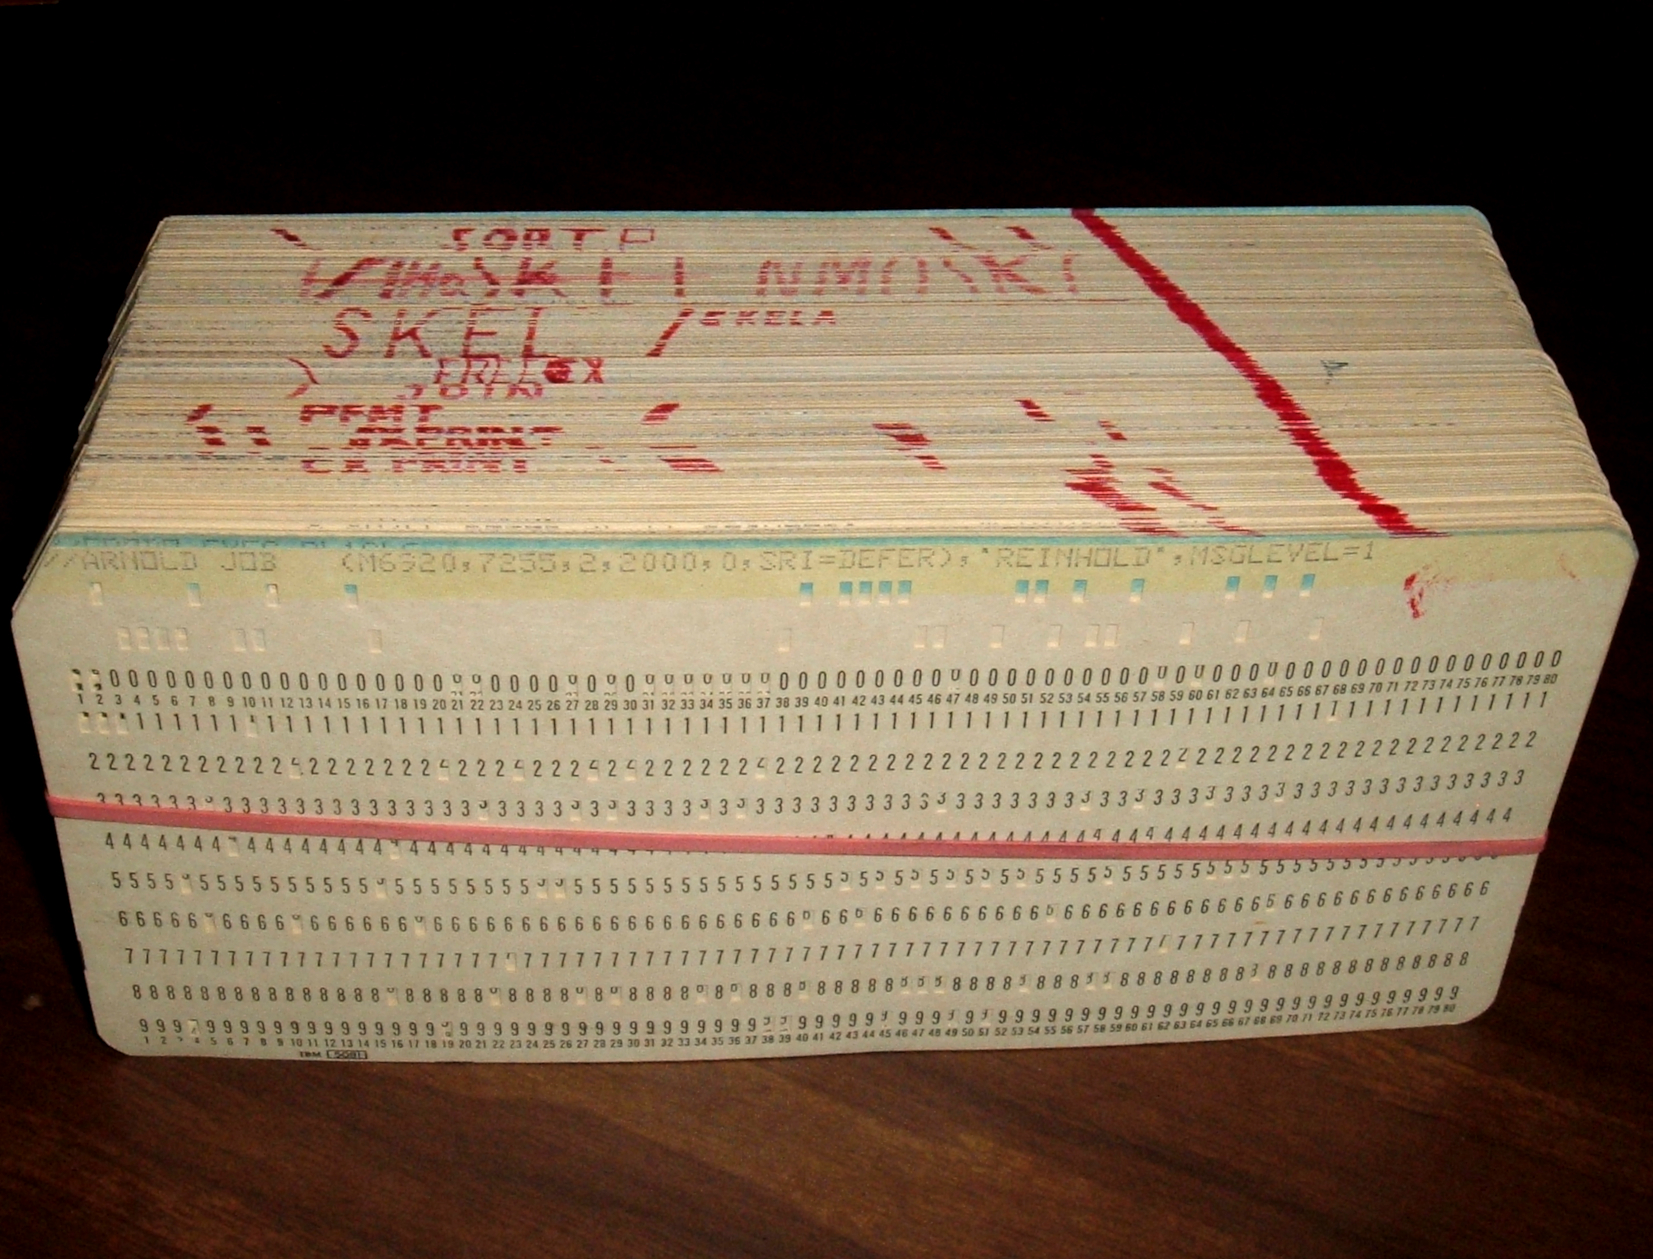
\includegraphics[height=0.7\textheight]{punched-cards}
        \end{centering}
    \end{figure}
\end{frame}

\begin{frame}
    \frametitle{Телетайп}
    \begin{minipage}{0.8\textwidth}
        \begin{figure}
            \begin{centering}
                % Credit: Wikipedia
                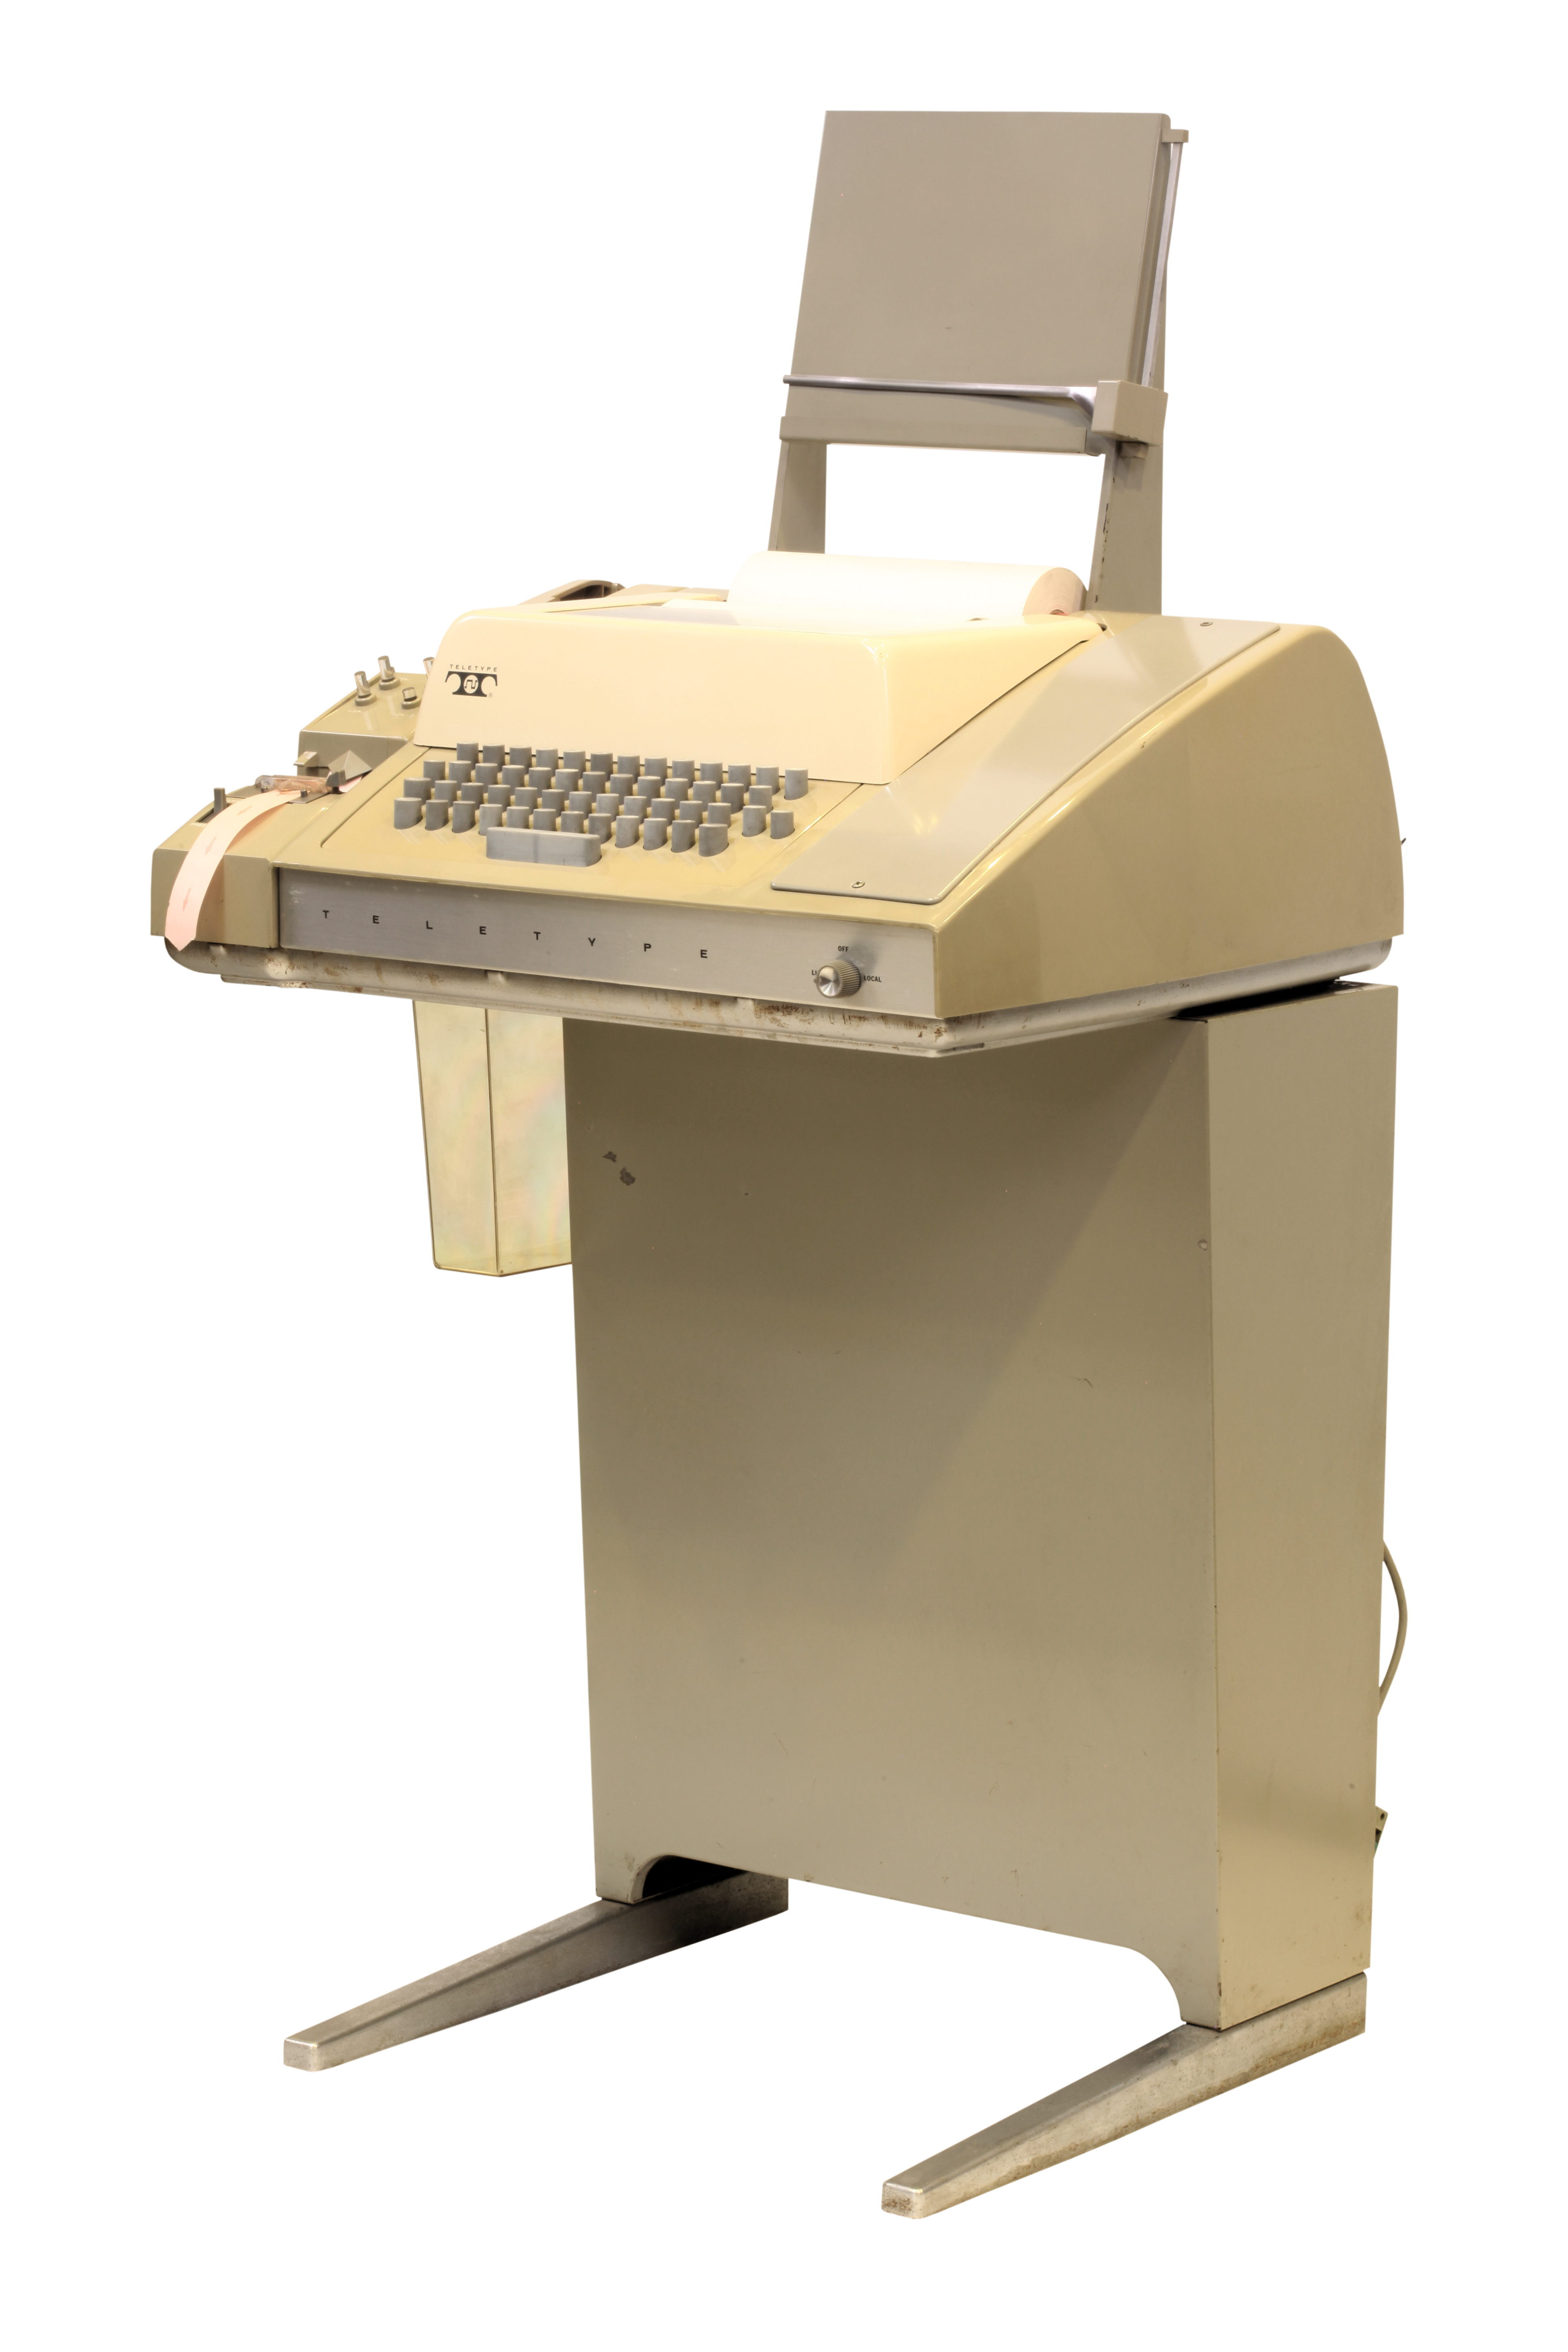
\includegraphics[height=0.8\textheight]{asr-33}
                \caption{ASR-33}
            \end{centering}
        \end{figure}
    \end{minipage}
    \begin{minipage}{0.19\textwidth}
        
\includegraphics[width=0.95\textwidth]{tty-qr}
    \end{minipage}
\end{frame}

\begin{frame}
    \frametitle{Терминал}
    \begin{figure}
        \begin{centering}
            %Credit: https://en.wikipedia.org/wiki/VT100
            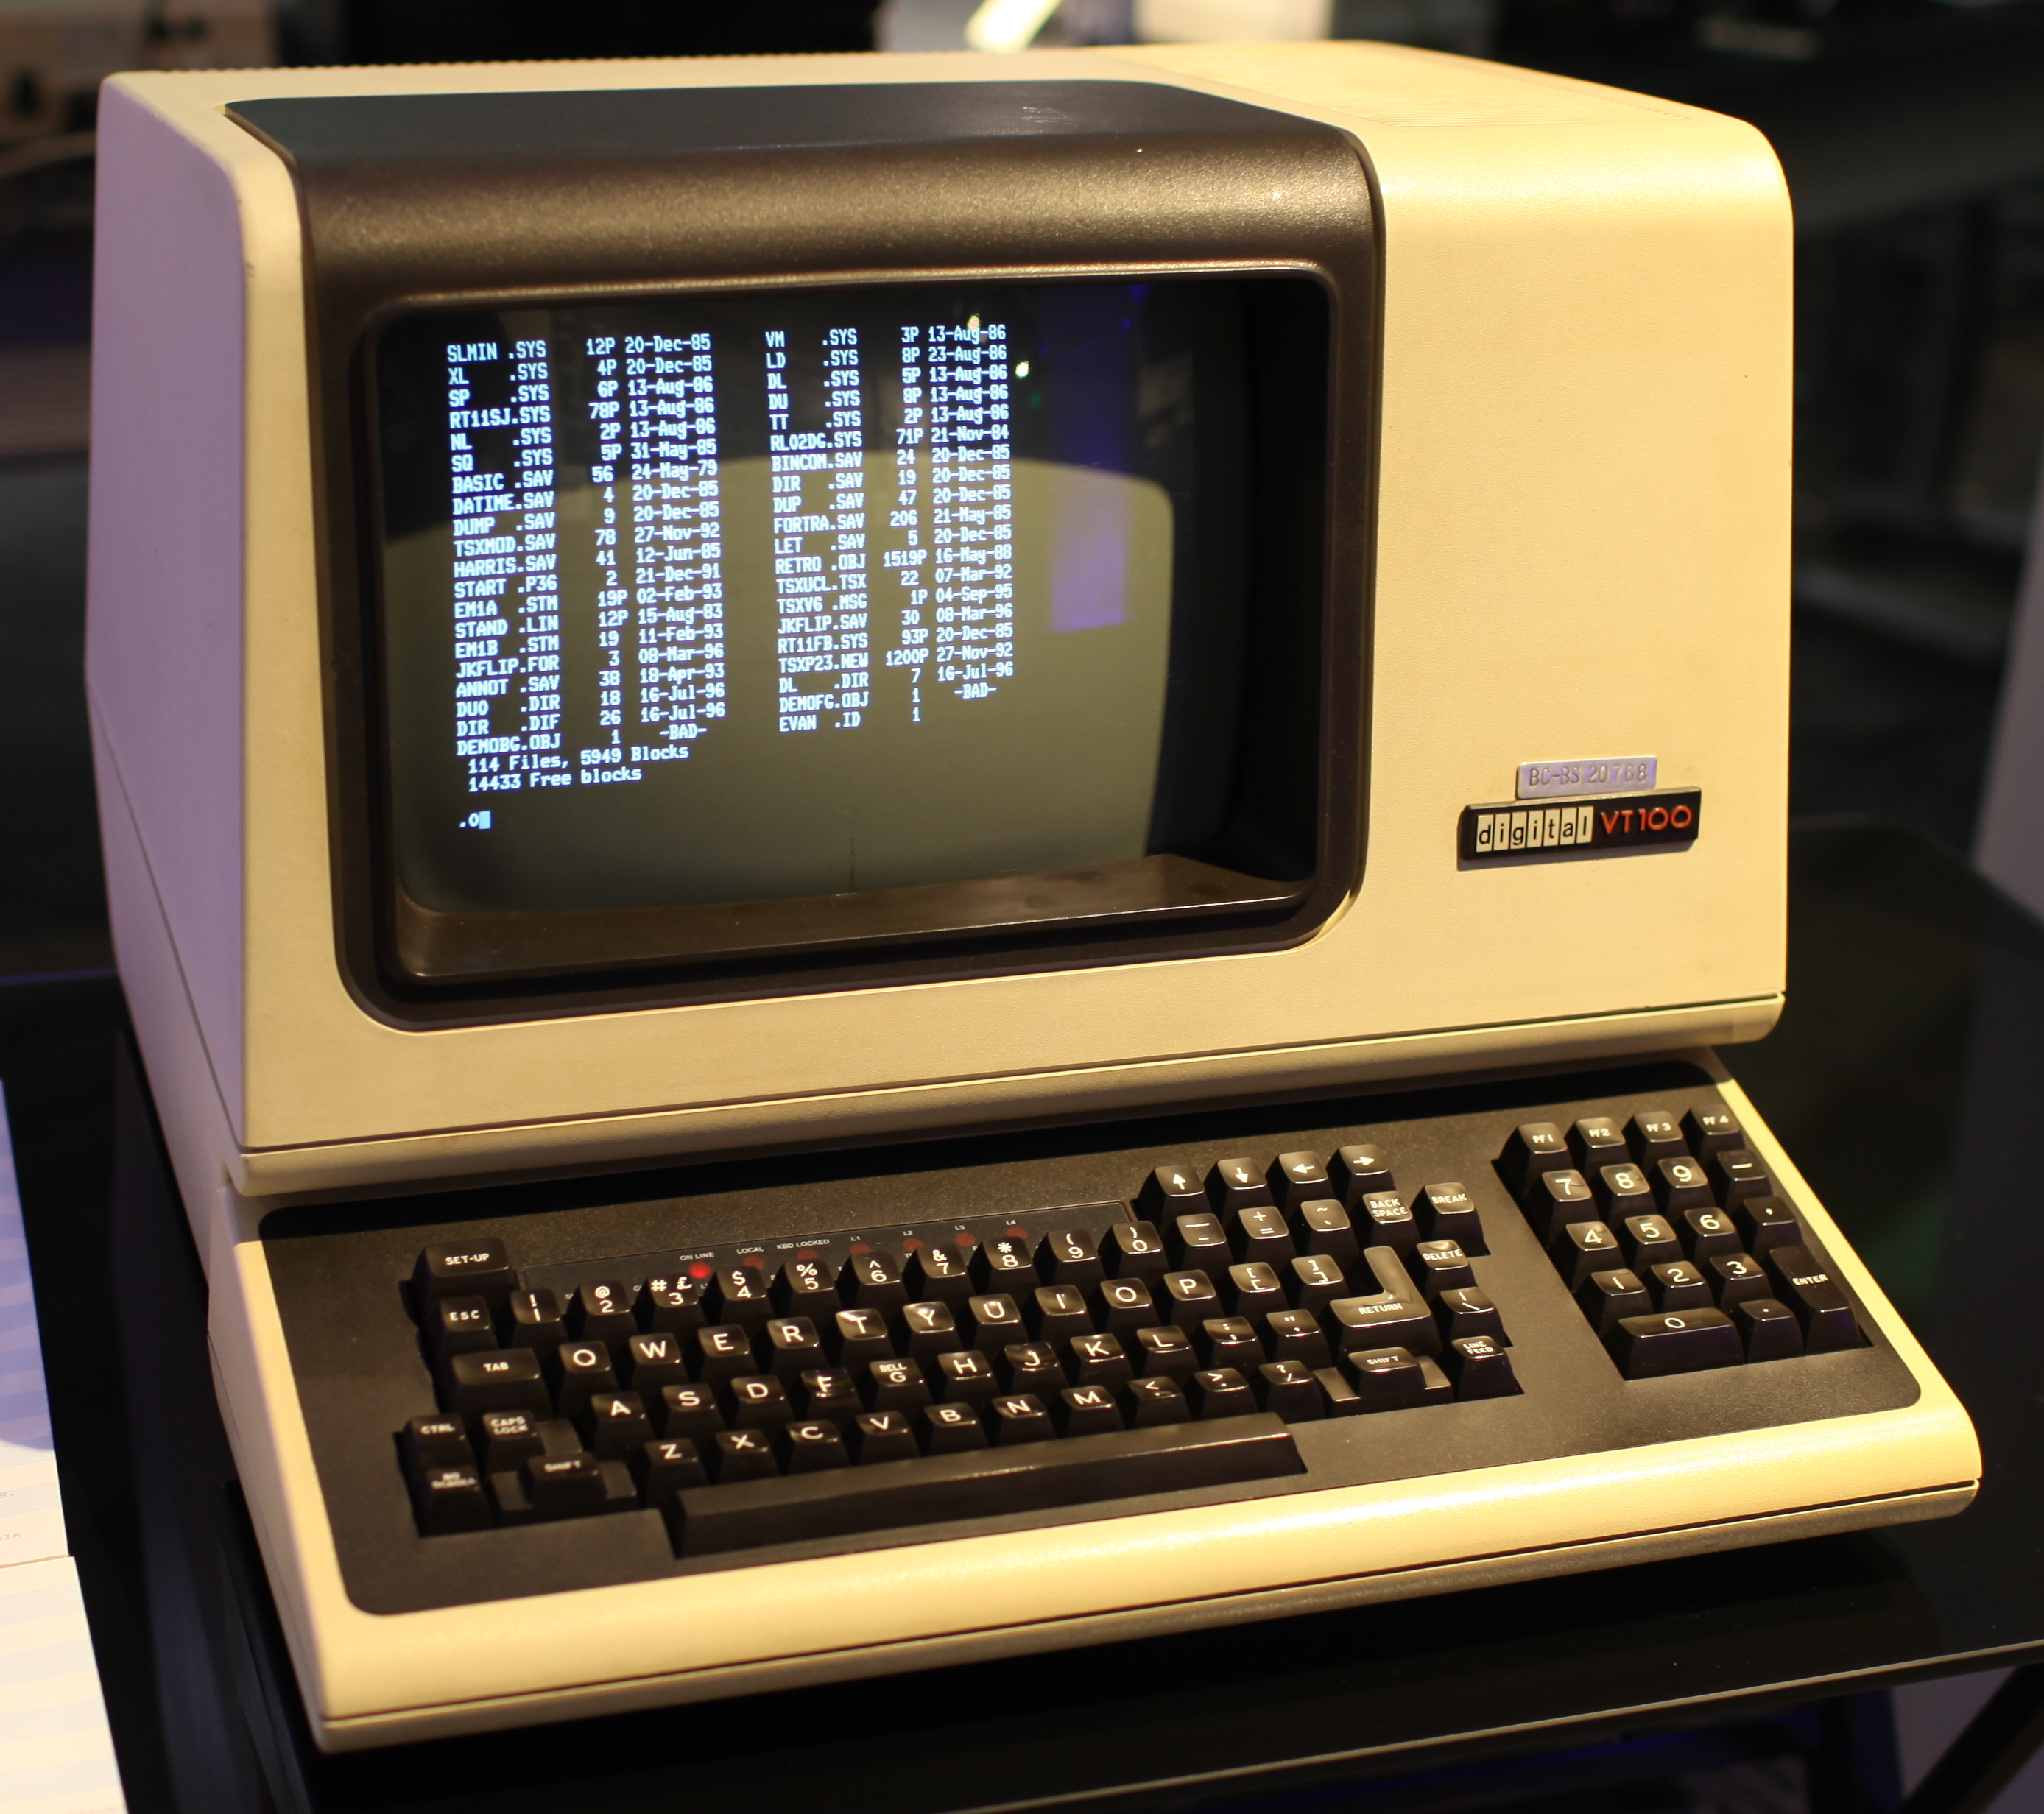
\includegraphics[height=0.7\textheight]{vt100}
            \caption{DEC VT-100}
        \end{centering}
    \end{figure}
\end{frame}

\section{Программы}
\begin{frame}
    \frametitle{Что такое программа?}
    \only<1->{
    Программа $=$ алгоритмы $+$ структуры данных
    }\only<2->{\par\vspace{0.5cm}
    Программы обычно записывают в виде текста на одном из \textit{языков
    программирования}
    }\only<3->{\par\vspace{0.5cm}
    Текст переводится в бинарный код \textit{транслятором}
    (\textit{компилятором}), или выполняется \textit{интерпретатором}
    }\only<4->{\par\vspace{0.5cm}
    Компилируемые языки программирования: \texttt{FORTRAN},
    \texttt{Algol}, \texttt{Pascal}, \texttt{C}, \texttt{C++}
    }\only<5->{\par\vspace{0.5cm}
    Интерпретируемые языки программирования: \texttt{shell},
    \texttt{perl}, \texttt{python}
    }\only<6->{\par\vspace{0.5cm}
    Библиотеки --- набор стандартных процедур с алгоритмами или с
    взаимодействием с операционной системой
    }
\end{frame}

\begin{frame}
    \frametitle{Операционные системы}
    \only<1->{
        Ядро операционной системы распределяет существующий ресурс
        <<железа>> между программами
    }\only<2->{\par\vspace{0.5cm}
    Ядро операционной системы предоставляет интерфейс к использованию
    <<железа>>
    }\only<3->{\par\vspace{0.5cm}
    В широком смысле операционная система --- это ядро плюс базовые
    системные программы и библиотеки, такие как командная оболочка
    (\texttt{shell}), программа инициализации при запуске, или
    стандартная библиотека языка Си
    }\only<4->{\par\vspace{0.5cm}
    Операционные системы могут быть \textit{self-hosted}: ядро и
    системные программы можно собрать из исходных текстов на самой
    операционной системе
    }
\end{frame}

\begin{frame}
    \frametitle{UNIX: предыстория}
    \only<1->{
        ОС MULTICS в шестидесятые годы: громоздкий проект трёх
        огромных американских организаций: General Electric, MIT, и AT\&T
    }\only<2->{\par\vspace{0.5cm}
    AT\&T решает, что MULTICS слишком сложна и не будет иметь
    коммерческого успеха, и выходит из коллаборации
    }\only<3->{\par\vspace{0.5cm}
    Нового задания для своих программистов из Bell Labs AT\&T не
    придумала
    }\only<4->{\par\vspace{0.5cm}
    Кен Томпсон и его коллеги играют в Space Travel
    }\only<5->{\par\vspace{0.5cm}
    Чтобы сделать игру дешевле, они решают портировать её на стоящий в
    углу, никому не нужный компьютер PDP-7
    }\only<6->{\par\vspace{0.5cm}
    Так зародилась ОС UNIX
    }
\end{frame}

\begin{frame}
    \frametitle{Ранний UNIX}
    \only<1->{
        Файл --- это просто поток байтов
    }\only<2->{\par\vspace{0.5cm}
    Иерархическая файловая система
    }\only<3->{\par\vspace{0.5cm}
    Процессорное время распределяется между пользователями
    }\only<4->{\par\vspace{0.5cm}
    Ядро написано на ассемблере (де-факто на машинных кодах)
    }
\end{frame}

\begin{frame}
    \frametitle{UNIX room}
    %Credit: https://twitter.com/rob_pike/status/896161131894419457
    \begin{figure}
        \begin{centering}
            \only<1>{
            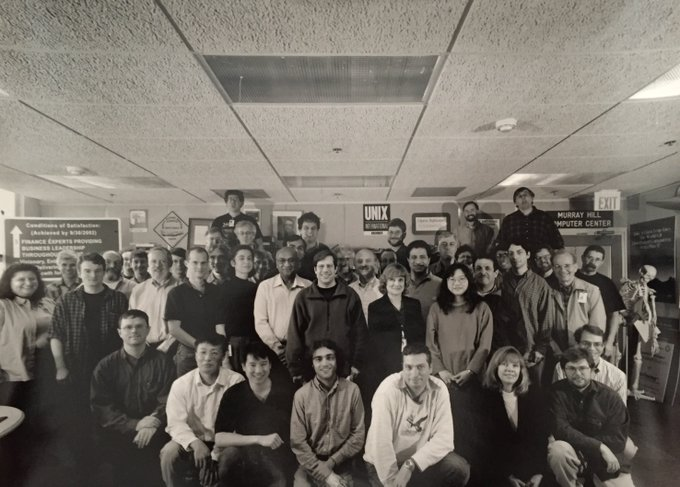
\includegraphics[height=0.7\textheight]{unix-room}
        }
            \only<2>{
                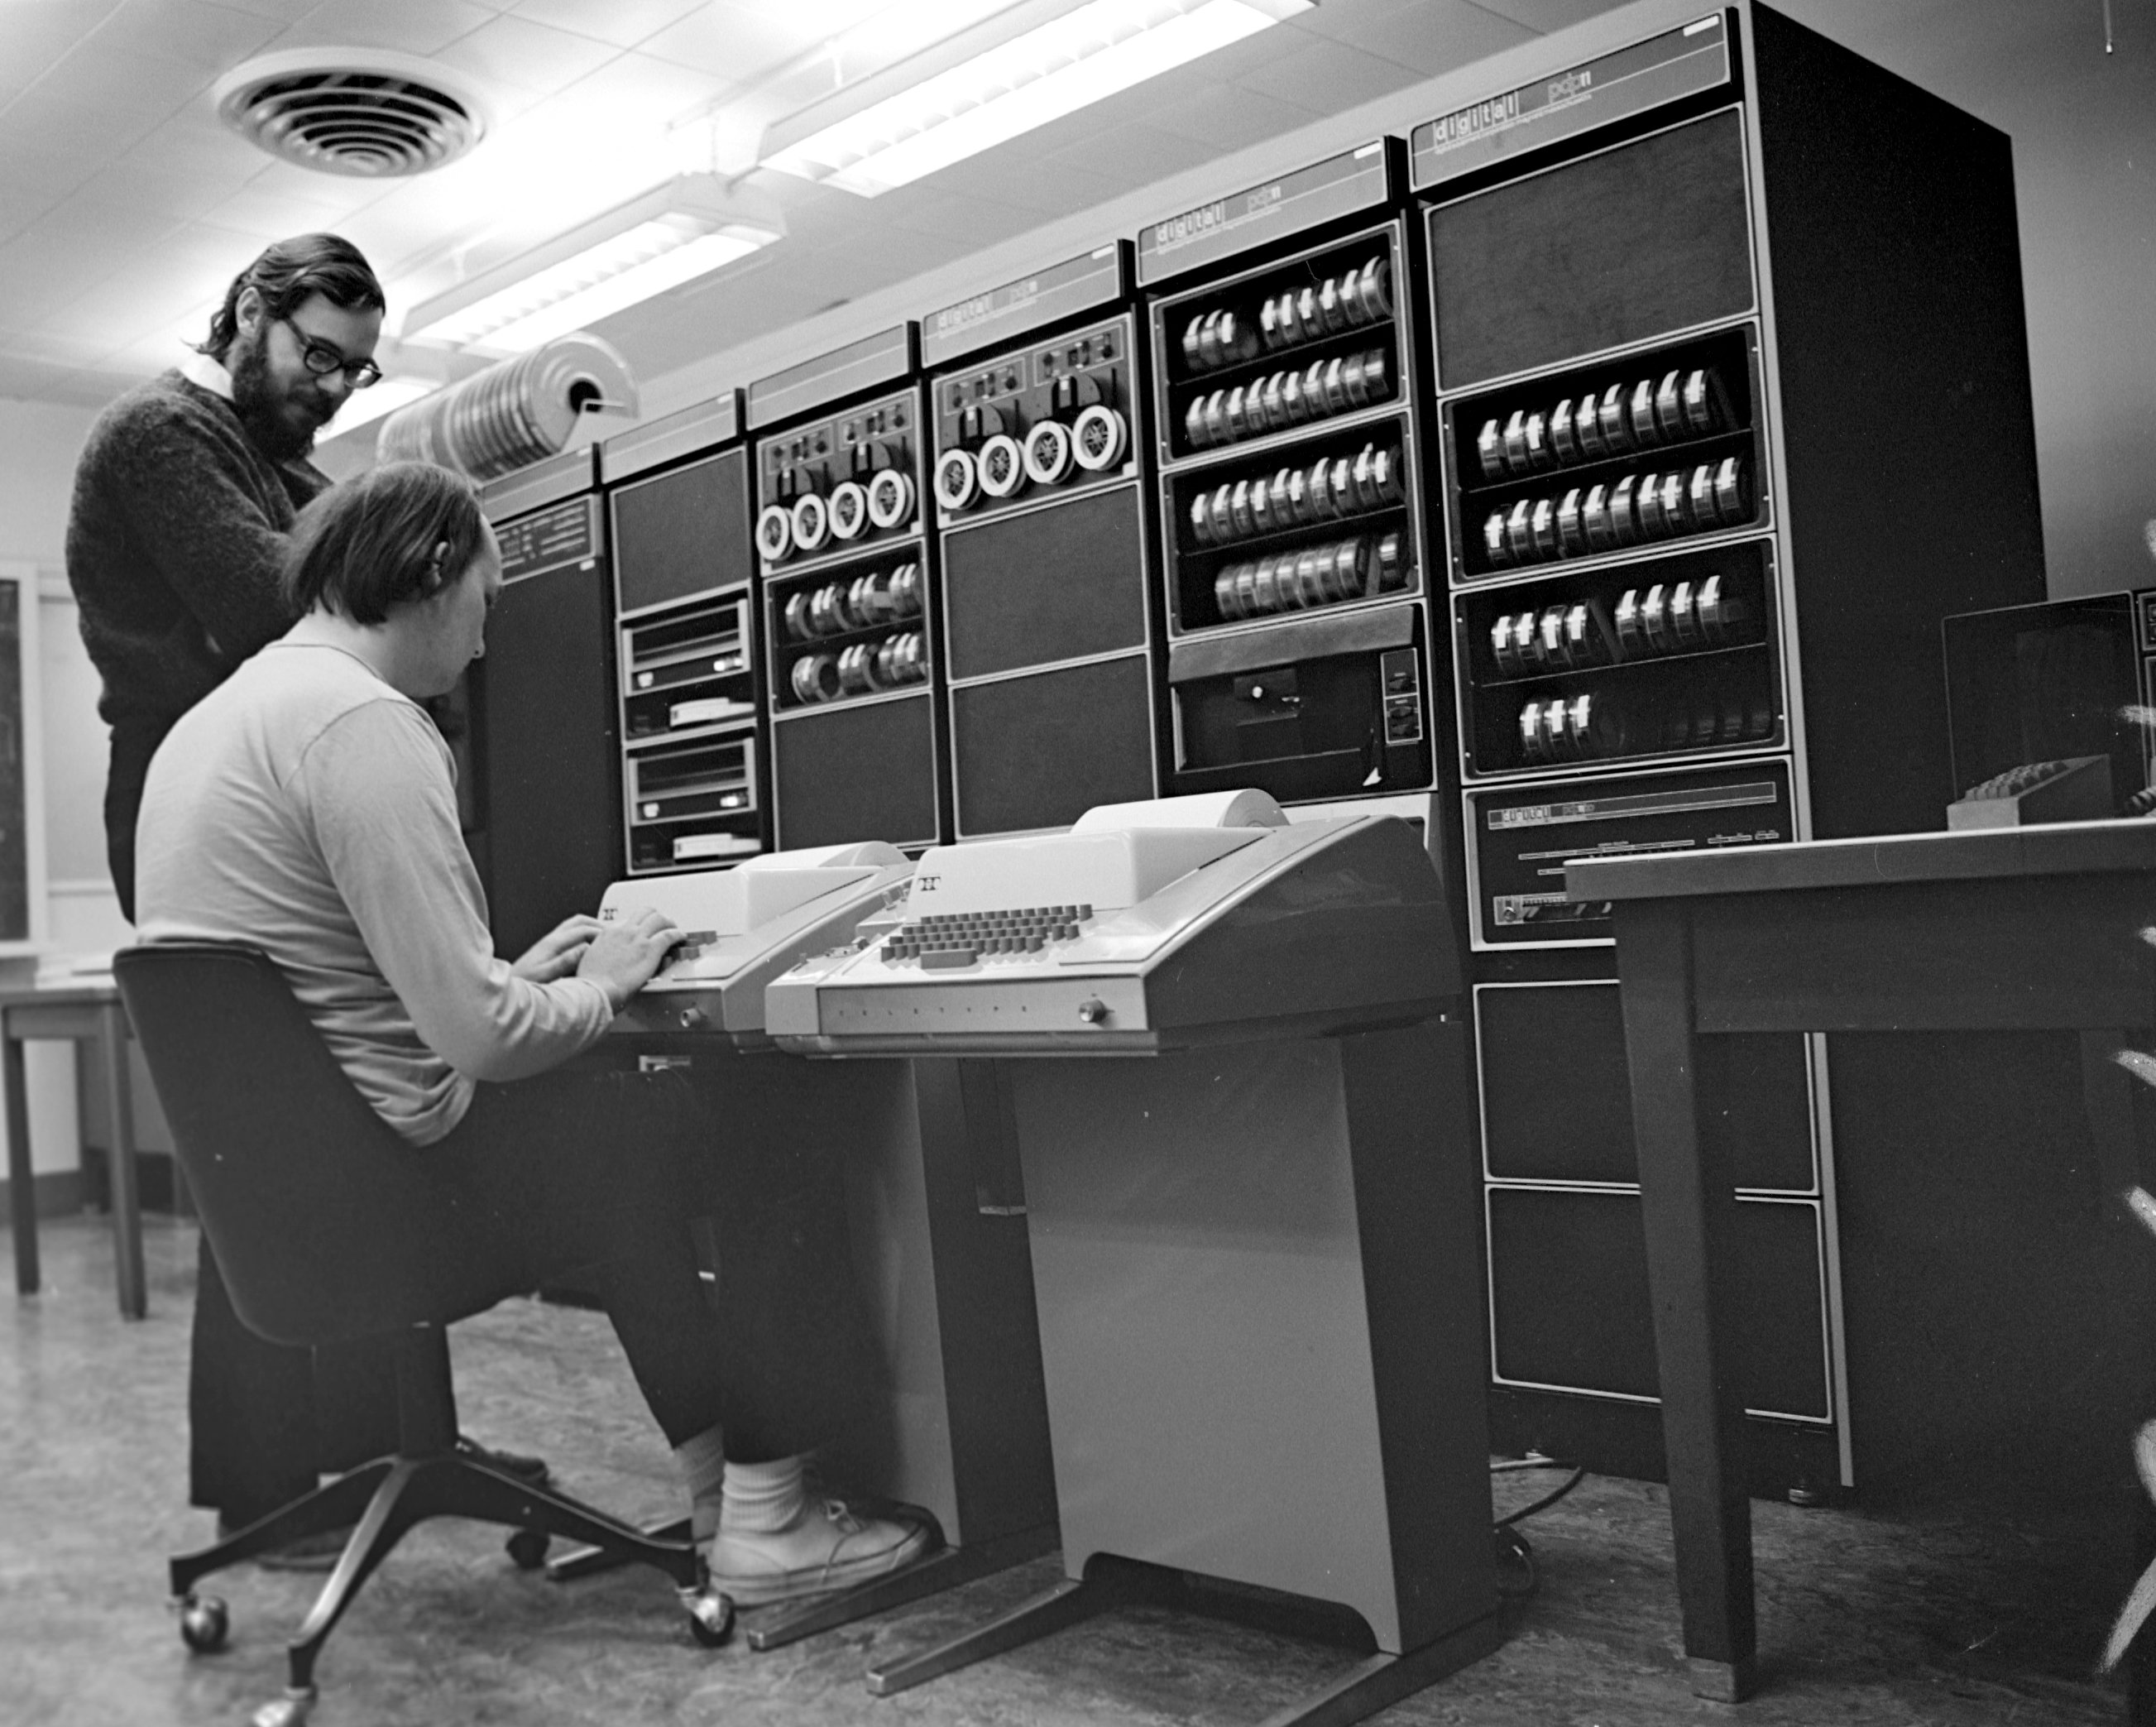
\includegraphics[height=0.7\textheight]{ken-dennis}
            }
        \end{centering}
    \end{figure}
\end{frame}

\begin{frame}
    \frametitle{Bell labs}
    \begin{figure}
        \begin{centering}
            %Credit: https://www.engadget.com/hitting-the-books-making-art-work-patrick-mc-cray-mit-press-163038701.html
            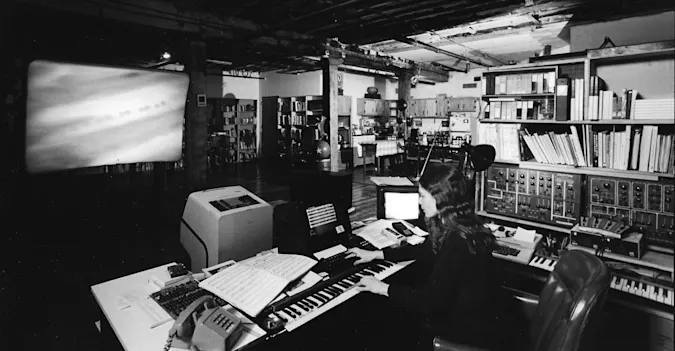
\includegraphics[height=0.7\textheight]{bell-labs}
        \end{centering}
    \end{figure}
\end{frame}

\begin{frame}
    \frametitle{Microsoft тоже использовали PDP-11}
    \begin{minipage}{0.8\textwidth}
        \begin{figure}
            \begin{centering}
                %Credit: Living computer museum, miss Piggy
                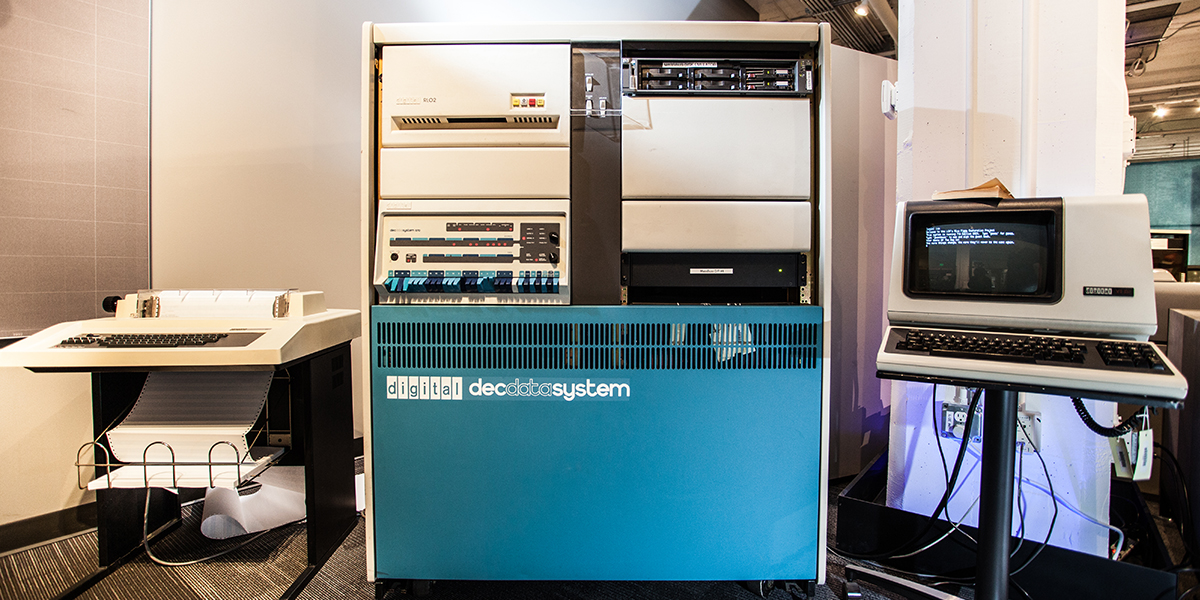
\includegraphics[height=0.7\textheight]{miss-piggy}
            \end{centering}
        \end{figure}
    \end{minipage}
    \begin{minipage}{0.19\textwidth}
        
\includegraphics[width=0.95\textwidth]{miss-piggy-qr}
    \end{minipage}
\end{frame}

\section{Лабораторные работы}
\begin{frame}
    \frametitle{Подготовка}
    \texttt{PuTTY} (Windows), \texttt{Termux} (Android)
    \par\vspace{0.25cm}
    \par\vspace{0.25cm}
    Проверка соединения: \texttt{ping IP\_ADDRESS}
    \par\vspace{0.25cm}
    Конфигурация терминала:
    \begin{itemize}
        \item Тип соединения: SSH
        \item IP: \texttt{IP\_ADDRESS}
        \item Порт: \texttt{22222}
    \end{itemize}
\end{frame}

\begin{frame}[fragile]
    \frametitle{Успешное соединение}
    \begin{verbatim}

ED25519 key fingerprint is SHA256:UOxq/SiPwFIxKUnZWnRqGnDJDAH0yoC1ivPSjdXrh/w.
This key is not known by any other names.
Are you sure you want to continue connecting (yes/no/[fingerprint])?
	\end{verbatim}
    Нужно ответить \texttt{yes} и нажать \texttt{Enter}
\begin{verbatim}
Warning: Permanently added 'HOSTNAME' (ED25519) to the list of known hosts.
(username@hostname) Password:
\end{verbatim}
    Введите ваш пароль. Он не будет печататься на экране.
\end{frame}

\begin{frame}
    \frametitle{Использование терминала}
    В UNIX терминальный ввод-вывод двусторонний: всё, что вы печатаете,
    отправляется систему, и в нормальном режиме отправляется обратно на
    экран терминала (\texttt{echo} режим).
    \par\vspace{0.25cm}
    За редким исключением: пароли
    \par\vspace{0.25cm}
    Введённые символы анализируются системой только при нажатии клавиши
    \texttt{RETURN} (на большинстве клавиатур: \texttt{Enter})
    \par\vspace{0.25cm}
    Другие специальные сигналы, которые терминал посылает ОС, кодируются
    с помощью одновременного нажатия на клавишу \texttt{CONTROL}
    (\texttt{Ctrl} на большинстве клавиатур); так, \texttt{\^}\texttt{M}
    эмулирует \texttt{RETURN}, \texttt{\^} означает \texttt{CONTROL}
\end{frame}

\begin{frame}
    \frametitle{Комбинации с \texttt{CONTROL}}
    \begin{tabular}{cl}
        \texttt{\^}\texttt{M} & \texttt{RETURN} \\
        \texttt{\^}\texttt{D} & Конец ввода \\
        \texttt{\^}\texttt{G} & Динь\\
        \texttt{\^}\texttt{H} & \texttt{Backspace}\\
        \texttt{\^}\texttt{I} & \texttt{TAB}\\
        \texttt{\^}\texttt{C} & Прерывание \\
        \texttt{\^}\texttt{S} & Остановить вывод \\
        \texttt{\^}\texttt{Q} & Восстановить вывод
    \end{tabular}
\end{frame}

\begin{frame}[fragile]
    \frametitle{Командная строка}
    Приветствие командной строки: \texttt{\$}
    \par\vspace{0.23cm}
    Команда не будет запущена до тех пор, пока клавиша \texttt{RETURN}
    (или \texttt{\^}\texttt{M}) не будет нажата
    \par\vspace{0.23cm}
    UNIX различает прописные и строчные буквы: \texttt{abcde} отличается
    от \texttt{ABCDE}
    \par\vspace{0.23cm}
    Вариант простой команды: \texttt{date} --- показать дату и время
    \par\vspace{0.23cm}
    Справка о командах: \texttt{man}. Например: \texttt{man man}
    \par\vspace{0.23cm}
    Ваше имя пользователя: \texttt{who am i}, или \texttt{who mom likes}
    \begin{verbatim}
[username@hostname:~]$ who am i
username terminal_device        date time
\end{verbatim}
    \par\vspace{0.23cm}
\end{frame}

\begin{frame}[fragile]
    \frametitle{Файловая система}
    Всё есть файл
    \par\vspace{0.25cm}
    Почти всё есть файл
    \par\vspace{0.25cm}
    Типы файлов: обычные, директории, специальные файлы устройств,
    \ldots
    \par\vspace{0.25cm}
\begin{verbatim}
localhost:~# pwd    # print current working directory
/root
localhost:~# cd /   # change directory (to the root "/")
localhost:/# pwd    # print currernt working directory
/
localhost:/# cd bin # change directory (to the bin)
localhost:/bin# ls echo # show list of files named echo
echo
\end{verbatim}
\end{frame}

\begin{frame}[fragile]
    \frametitle{Файловая система}
    \begin{verbatim}
# ls -l
total 52
drwxr-xr-x    2 root     root          2089 Jan  9  2021 bin
drwxr-xr-x    4 root     root          2240 Mar 28 11:04 dev
drwxr-xr-x   39 root     root          1979 Jan  9  2021 etc
drwxr-xr-x    2 root     root            37 Jul  5  2020 home
drwxr-xr-x    8 root     root           901 Aug 17  2020 lib
drwxr-xr-x    2 root     root            37 May 29  2020 mnt
dr-xr-xr-x   12 root     root             0 Mar 28 11:04 sys
drwxrwxrwt    2 root     root            37 Jan  9  2021 tmp
drwxr-xr-x   10 root     root           229 Jun 24  2020 usr
drwxr-xr-x   16 root     root           348 Aug 27  2020 var
\end{verbatim}
\end{frame}

\begin{frame}[fragile]
    \frametitle{Файловая система}
\tikzstyle{every node}=[draw=black,thick,anchor=west]
\tikzstyle{selected}=[draw=red,fill=red!30]
\tikzstyle{optional}=[dashed,fill=gray!50]
\begin{tikzpicture}[%
  grow via three points={one child at (0.5,-0.7) and
  two children at (0.5,-0.7) and (0.5,-1.4)},
  edge from parent path={(\tikzparentnode.south) |- (\tikzchildnode.west)}]
  \node {texmf}
    child { node {doc}}		
    child { node {fonts}}
    child { node {source}}
    child { node [selected] {tex}
      child { node {generic}}
      child { node [optional] {latex}}
      child { node {plain}}
    }
    child [missing] {}				
    child [missing] {}				
    child [missing] {}				
    child { node {texdoc}};
\end{tikzpicture}
\end{frame}

\begin{frame}[fragile]
    \frametitle{Текстовый редактор}
    \begin{verbatim}
[username@hostname]$ ed
a
some junk
even more junk
more and more
.
w
?
w junk
39
q
[username@hostname]$
\end{verbatim}
\end{frame}

\begin{frame}[fragile]
    \frametitle{Текстовый редактор}
    \begin{verbatim}
[username@hostname]$ cat junk
some junk
even more junk
more and more
\end{verbatim}
    Более мощный редактор: VIsual Improved (\texttt{vim})
\begin{verbatim}
vimtutor uk # украинская версия
vimtutor ru # русская версия
\end{verbatim}
\end{frame}

\begin{frame}
    \frametitle{План занятий}
    \only<1->{
        Основы языка Си
    }\only<2->{\par\vspace{0.2cm}
        Проектная работа
        \begin{itemize}[<+->]
            \item Веб-форум
            \item Макетный компьютер
            \item Операционная система
            \item Компилятор Си
            \item Олимпиадное программирование
        \end{itemize}
        }
\end{frame}

\begin{frame}
    \frametitle{Полезные ссылки}
    \begin{columns}
        \begin{column}{0.5\textwidth}
            \begin{tabular}{l c}
                Druzi prog веб-страница: &
                
\includegraphics[width=0.24\textwidth]{druzi-prog}\\
                \texttt{vimtutor.uk} &
                
\includegraphics[width=0.24\textwidth]{vimtutor.uk}\\
                \texttt{vimtutor.ru} &
                
\includegraphics[width=0.24\textwidth]{vimtutor.ru}\\
            \end{tabular}
        \end{column}
        \begin{column}{0.5\textwidth}
            \begin{tabular}{l c}
                Хакеры Druzi телеграм-группа: &
                
\includegraphics[width=0.24\textwidth]{tg-qr}\\
            \end{tabular}
        \end{column}
    \end{columns}
\end{frame}

\end{document}
